\documentclass[11pt]{article}
\usepackage[margin=1in]{geometry}
\usepackage{amsmath,amssymb,graphicx,xcolor,booktabs,microtype,enumitem}
\usepackage[labelfont=bf,font=small]{caption}
\usepackage{mathpazo}
\usepackage[colorlinks=true,linkcolor=blue!55!black,citecolor=blue!55!black,urlcolor=blue!55!black]{hyperref}
\usepackage{tikz}
\usetikzlibrary{arrows.meta,decorations.pathreplacing}
\definecolor{acc}{HTML}{2c5aa0}
\newcommand{\dg}{^{\dagger}}
\newcommand{\ip}[2]{\langle #1,\,#2\rangle}
\newcommand{\E}{\mathbb{E}}
\setlist{itemsep=2pt,topsep=3pt}
\newtheorem{claim}{Claim}
\newtheorem{prop}{Proposition}
\usepackage{cite}

\title{\vspace{-1.2cm}Adjoint Transport Theory for Rare-Event Sampling in Spin
		Systems\\[2pt]
	\large A tested implementation: what the transport--statistical-mechanics
	correspondence buys, and what it does not}
\author{}\date{}

\begin{document}
	\maketitle
	\vspace{-1.3cm}
	\begin{center}\rule{0.62\textwidth}{0.4pt}\end{center}
	
	\begin{abstract}
		\noindent Radiation transport solved rare-event sampling decades ago with the adjoint
		importance function and the CADIS/weight-window machinery, a quantity that turns out to
		be mathematically identical to the rare-event committor of Markov chain theory. We
		transfer this toolkit to statistical mechanics and test it end to end on the 2D Ising
		ferromagnet and the Edwards--Anderson spin glass, asking which parts of it actually earn
		their keep. The adjoint-committor identity is exact, verified here to machine precision,
		and Weighted Ensemble sampling (weight windows applied to spin configurations) reaches
		two decades deeper into the tail than naive Monte Carlo at matched cost. A learned
		importance coordinate trained on a milestoning surrogate label does not beat a
		hand-picked energy coordinate. An ensemble of independently-trained networks, built to
		resolve an earlier ambiguous result, instead converges on a statistically decisive loss
		(FOM ratio $0.087\times$, 95\% CI $[0.051,0.155]$). Every comparison up to that point,
		though, was run at a depth where naive Monte Carlo still holds its own. Tested at a depth
		calibrated so naive is provably blind, a self-consistency training objective shaped
		directly on the harmonic committor condition, rather than an energy-adjacent proxy of it,
		finds the rare event significantly more often than the hand-picked coordinate ($66.7\%$
		vs.\ $40.0\%$ hit rate across three independent networks, $p=0.017$), though a matching
		cost-efficiency advantage has not yet been established. A global variance-reduction
		objective (FW-CADIS) matches uniform allocation's error profile at one-eighth the cost,
		but does not flatten relative error the way it is meant to. Naive Monte Carlo is not
		beaten outright at any lattice size tested ($L=8$--$32$) at shallow threshold depths.
		Together, these results say the transport toolkit's value is concentrated in the
		genuinely rare regime it was built for, and depends on a training objective shaped like
		the true committor rather than a convenient proxy of it.
	\end{abstract}
	
	\section{Introduction}
	\label{sec:intro}
	
	The application domains on the statistical-mechanics side are not hypothetical: Weighted Ensemble, Forward Flux Sampling, and committer-based
	methods are already the working tools for nucleation and crystallization, protein folding
	and conformational transitions, and chemical reaction rates via transition-state theory
	\cite{allen2009, zuckerman2017, e2006}. A transport toolkit that reliably picks the
	importance function for them, rather than requiring a hand-chosen progress coordinate,
	would apply directly to that existing user base. The obstacle is structural, since an unbiased estimator of an
	event of probability $p$ has relative error of order $(Np)^{-1/2}$, so each decade of
	rarity costs an order of magnitude in computing \cite{allen2009, touchette2009}. Every
	serious remedy therefore replaces more samples with samples drawn, an idea present in Monte Carlo since importance sampling and trajectory splitting \cite{kahn1951, kahn1953}.
	
	Radiation transport met the problem first, in deep-penetration shielding, where analog
	scoring probabilities fall below $10^{-10}$ \cite{spanier1969, wagner1998}. Its remedy is
	the \emph{adjoint} flux, or importance function, which runs the transport equation
	backwards from the detector response and measures the expected contribution of a particle
	at each phase-space point \cite{lewins1965, bell1970}. An importance function so obtained
	is used both to bias source emission and to set weight windows, inside which particles are
	split and outside which they are killed by Russian roulette \cite{kahn1951, booth1984}.
	CADIS automated this by deriving source biasing and weight windows consistently from a
	coarse deterministic adjoint, giving figure-of-merit gains of several orders of magnitude
	on realistic geometries \cite{wagner1998, haghighat2003}; its forward-weighted extension
	FW-CADIS replaces the single-detector objective with a \emph{global} one, seeking uniform
	uncertainty across a whole family of responses \cite{wagnerfw2014, cooper2001}.
	Throughout, performance is judged by the figure of merit
	$\mathrm{FOM}=1/(\sigma_{\mathrm{rel}}^{2}T)$, a cost-normalised inverse variance
	\cite{spanier1969, wagnerfw2014}.
	Transition Path Theory describes the statistics of reactive trajectories through the probability of reaching a target set before returning to the origin set (the committor)	$h(s)$, which
	is the optimal reaction coordinate in a precise sense \cite{e2006, metzner2009,
		evanden2010}. Its practical samplers are splitting methods in disguise: Weighted Ensemble
	splits and merges weighted replicas across bins in a progress coordinate \cite{huber1996},
	a scheme later shown statistically exact for broad classes of processes and binnings
	\cite{zhang2010}; Forward Flux Sampling and Adaptive Multilevel Splitting advance an
	ensemble through fixed or adaptive interfaces \cite{allen2009, cerou2007}; and Transition
	Path Sampling works directly in trajectory space \cite{bolhuis2002}. What unites and
	limits them all is dependence on a user-supplied coordinate, with no general prescription
	for choosing it \cite{zuckerman2017, allen2009}. Lattice spins are the natural testbed:
	the 2D Ising ferromagnet \cite{ising1925} has an exact solution to validate against
	\cite{onsager1944}, while the Edwards--Anderson model adds quenched disorder, frustration
	and no obvious coordinate \cite{edwards1975, binder1986}. Both are usually simulated with
	Metropolis dynamics \cite{metropolis1953}, whose critical slowing down motivated cluster
	updates \cite{swendsen1987, wolff1989} and flat-histogram schemes \cite{berg1992,
		wanglandau2001}, methods that flatten a free-energy landscape rather than steer
	trajectories toward a specified tally, and so optimise a mismatched objective here
	\cite{wanglandau2001}.
	
	The identity between the two is classical rather than new. Both objects are instances of
	Doob's $h$-transform, which conditions a process on a rare terminal event by tilting its
	generator with the corresponding harmonic function \cite{doob1984}; the same construction
	reappears as the driven process of large-deviation theory and underpins the zero-variance
	sampler \cite{chetrite2015, touchette2009}, and again in stochastic-control form as the
	solution of a Gibbs variational principle \cite{hartmann2019}. Machine learning has since
	supplied a third route: physics-informed networks solve high-dimensional PDEs without a
	grid \cite{raissi2019}, and this was applied to the committor equation itself
	\cite{li2019, khoo2019}, with active importance sampling added to concentrate training
	effort where the loss is dominated by rarely visited regions \cite{rotskoff2020}. A
	separate, active line trains a committor variationally and uses it as a metadynamics-like
	collective variable with a transition-state-oriented bias potential, rather than a
	weight-window schedule, to sample molecular rare events uniformly across competing
	pathways \cite{trizio2025}, methodologically distinct from the splitting/rouletting
	machinery this paper transfers, though the same underlying object.
	Generative models were meanwhile trained directly on spin systems: variational
	autoregressive networks \cite{wu2019} and Boltzmann generators \cite{noe2019}, with
	later work recovering unbiased observables by reweighting \cite{nicoli2020} or embedding
	the model in a Markov chain \cite{gabrie2022}. Closest to this work, a recent preprint
	learns an importance function on a discrete chain from a label-free self-consistency
	objective and explicitly identifies adjoint flux with committor \cite{kim2026}.
	
	The gap this leaves is specific. The identity is established \cite{doob1984, chetrite2015}
	and neural committors exist \cite{li2019, khoo2019, kim2026, trizio2025}, but the transport
	\emph{toolkit} built around that identity (consistent weight windows, the global
	FW-CADIS objective, the figure of merit as an evaluation standard) was designed for
	precisely the regime where learned-committor methods are weakest \cite{wagner1998,
		wagnerfw2014}, and has never been transferred to spin systems and audited: every
	neural-committor line above samples by continuously reweighting or biasing dynamics, not
	by the transport toolkit's discrete population control (splitting, roulette, resampling
	to a fixed per-bin occupancy), so that mechanism and its FOM/FW-CADIS evaluation standard
	remain untested here. That is the project reported here, summarised in three claims:
	\begin{enumerate}[itemsep=2pt]
		\item The optimal importance function for a rare tally \emph{is} the committor, and
		tilting by the exact committor is zero-variance \cite{doob1984, chetrite2015}.
		\item CADIS/FW-CADIS weight windows can tame the fragility of an imperfect importance
		estimate and, in the global form, flatten relative error across a family of rare
		thresholds \cite{wagner1998, wagnerfw2014}.
		\item The FOM is a principled evaluation metric and a natural training objective,
		aligned with variance reduction rather than with free-energy surrogates
		\cite{spanier1969, wanglandau2001}.
	\end{enumerate}
	
	We test each of these three claims end to end on the 2D Ising ferromagnet and the
	Edwards--Anderson spin glass, treating each piece of machinery as a hypothesis rather than
	a technique to be demonstrated. Claim~(i) holds to numerical precision; claims~(ii) and
	(iii) proved more interesting, since several apparent wins did \emph{not} survive a proper
	bootstrap confidence interval, and the paper's one result that did survive such scrutiny
	only became significant once the target was pushed rare enough that naive Monte Carlo
	could no longer compete at all. \S\ref{sec:results} reports every comparison in full.

	\section{Theory: the adjoint$=$committor identity}
	\label{sec:theory}
	
	\subsection{Linear transport and the adjoint importance function}
	Let $P=(\mathbf r,\mathbf\Omega,E)$ be a phase-space point and $\psi(P)$ the particle flux
	obeying the linear transport (Boltzmann) equation, written abstractly as $\mathcal H\,\psi
	= q$, with transport operator $\mathcal H$ (streaming $+$ collision) and source $q$. A
	detector response (``tally'') is a linear functional $R=\ip{\sigma_d}{\psi}=\int
	\sigma_d(P)\,\psi(P)\,dP$, where $\sigma_d$ is the detector cross-section. Define the
	\emph{adjoint} flux $\psi\dg$ by
	\begin{equation}
		\mathcal H\dg\,\psi\dg=\sigma_d .
		\label{eq:adjoint}
	\end{equation}
	The defining property of the adjoint gives the fundamental identity
	\begin{equation}
		\boxed{\;R=\ip{\sigma_d}{\psi}=\ip{\psi\dg}{q}\;}
		\label{eq:fund}
	\end{equation}
	and the physical reading that makes everything work: $\psi\dg(P)$ is the expected
	contribution to the tally $R$ of a single particle introduced at $P$, its
	\emph{importance}. If one samples particle transitions biased toward high importance and
	assigns each particle the statistical weight $w(P)\propto 1/\psi\dg(P)$, then, when
	$\psi\dg$ is exact, every history contributes an identical score and the estimator of $R$
	has \emph{zero variance}. This is the theoretical ceiling of variance reduction; all
	practical schemes approximate it.
	
	\subsection{CADIS, FW-CADIS, weight windows, figure of merit}
	Since $\psi\dg$ is unknown, CADIS (Consistent Adjoint-Driven Importance Sampling) computes
	a cheap, approximate $\psi\dg$ and uses it to drive an expensive forward Monte Carlo run
	through two consistent devices: source biasing, sampling from
	$\hat q(P)=\psi\dg(P)q(P)/R$ instead of $q$; and weight windows, assigning each
	phase-space cell a target weight $w\propto 1/\psi\dg$ and a window
	$[w_{\text{target}}/k,\,k\,w_{\text{target}}]$: a particle above the window is
	\emph{split} into equal-weight copies, one below is \emph{Russian-rouletted}. This keeps
	$w(P)\,\psi\dg(P)\approx\text{const}$, bounding the weight and hence the variance.
	FW-CADIS (forward-weighted CADIS) extends this to \emph{global} variance
	reduction: weighting the adjoint source by the inverse of the local forward response
	produces weight windows that equalise \emph{relative} statistical error across many
	detectors, or the whole domain, at once, rather than optimising a single tally. Efficiency
	is measured by the figure of merit $\mathrm{FOM}=1/(\sigma_{\mathrm{rel}}^2\,T)$, the
	inverse product of relative variance and CPU time.
	
	\subsection{The central identity: importance $=$ committor $=$ zero-variance measure}
	\label{sec:identity}
	Work with a Markov chain on configurations $s$ with transition kernel $K(s\to s')$. Let $A$
	(failure/bulk) and $B$ (the rare target set) be disjoint, and define the committor
	$h(s)=\Pr[\text{reach }B\text{ before }A\mid\text{start at }s]$, with $h|_A=0$, $h|_B=1$.
	On the transient set it satisfies the discrete backward equation
	\begin{equation}
		h(s)=\sum_{s'}K(s\to s')\,h(s')\qquad\Longleftrightarrow\qquad (\mathbb I-K)\,h=0 .
		\label{eq:committor}
	\end{equation}
	Equation~\eqref{eq:committor} is precisely the discrete adjoint transport
	equation~\eqref{eq:adjoint} with the target set playing the role of the detector. Hence the
	rare-event committor $h(s)$, the transport adjoint importance $\psi\dg(s)$ (with
	$\sigma_d=\mathbf 1_B$), and the ``neural importance function'' of recent ML papers are the
	same function: the expected contribution of a walker at $s$ to the rare tally. Defining the
	tilted kernel $\widetilde K(s\to s')=K(s\to s')\,h(s')/h(s)$, the path likelihood ratio
	telescopes to $W=h(s_0)/h(s_{\text{end}})=h(s_0)$ for every path ending in $B$: every sample
	returns the identical value $h(s_0)=\pi$, so the estimator of $\pi$ has zero variance.
	This is why tilting helps: it converts the free-energy barrier the untilted walk has to
	climb into a downhill drift along the committor.

	Two readings of $\pi$ are possible here, and this paper always means the second. The
	\emph{static} equilibrium mass $\Pr_{\rm eq}(s\in B)=\sum_{s\in B}p(s)$ is a property of the
	stationary measure alone, answerable by direct enumeration with no dynamics at all: our
	$L=4$ gate (\S\ref{sec:res-we}) computes exactly this. The \emph{dynamical} hitting
	probability $h(s_0)$ from a fixed bulk reference state $s_0\in A$ is a different object: it
	is what every $\hat\pi$ reported in \S\ref{sec:results} actually estimates, and what
	Weighted Ensemble is built to sample efficiently. The two coincide under the same mixing
	condition transition-path theory already requires \cite{e2006}: dynamics equilibrates
	within $A$ faster than it escapes toward $B$, true throughout the $T=2.6>T_c$ regime tested
	here but not guaranteed at low temperature, where $A$ could itself fragment into
	sub-basins.

	This was verified directly on a solvable 1D toy walk before any spin-system code was
	written: tilting with the \emph{exact} committor gave measured relative variance
	$\sim\!10^{-30}$ (zero to machine precision), while tilting with an \emph{approximate}
	committor under pure biasing (no split/roulette) was \emph{worse than plain naive Monte
		Carlo}. That fragility is exactly why deep-penetration transport uses weight windows to
	bound the weights rather than relying on reweighting alone, and it is the reason every
	learned-coordinate result in this paper uses Weighted Ensemble, not pure importance
	reweighting.

	\subsection{Scope of the correspondence}
	\label{sec:scope}
	The identity above is exact at the level of linear algebra, not merely structurally
	similar, and it is worth stating precisely how far that goes. Production transport codes
	do not solve the continuous operator equation~\eqref{eq:adjoint} directly: phase space is
	first discretized into energy groups and a finite set of directions
	\cite{wagner1998, lewins1965}, reducing it to a finite linear system
	$(\mathbb I-\mathbf K)\boldsymbol\psi\dg=\boldsymbol\sigma_d$ for a transition operator
	$\mathbf K$ packaging streaming and scattering between cells, term for term the same
	system as Eq.~\eqref{eq:committor}. Nothing about $K$'s physical origin enters that algebra,
	which is exactly why the identity transfers to spin dynamics with no modification to the
	mathematics: it holds for \emph{any} Markov process with an absorbing target set.

	What does not transfer is the physical mechanism generating $K$. Transport's $K$ encodes a
	particle's free flight interrupted by scattering and absorption at rates set by
	cross-sections; spin dynamics' $K$ encodes single-spin-flip acceptance under a thermal bath
	at temperature $T$. There is no mean free path or cross-section in the spin problem, and a
	``walker'' is a bookkeeping device for one member of a population of independent
	simulation replicas, not a physical particle. The correspondence is a shared
	mathematical structure, not a shared physical mechanism.

	Two asymmetries follow, in opposite directions. Spin systems are the \emph{easier} problem
	in one specific sense: multigroup/discrete-ordinates transport carries a discretization
	error that must be checked against measurement, since the exact continuous answer is rarely
	available at all, whereas a spin lattice's state space is already finite
	($2^N$ configurations, no truncation), which is exactly why $L=4$ can be checked against
	exact enumeration directly (\S\ref{sec:res-we}) with no discretization step to introduce
	error. Spin systems are \emph{harder} in the place it matters most: transport bins its
	importance function along a natural, low-dimensional, physically meaningful coordinate
	(position, direction, energy, fixed by the geometry of the shield), while spin
	configurations have no such coordinate (\S\ref{sec:models} shows the obvious candidate,
	magnetization, fails outright on the spin glass). That absence, not the linear algebra, is
	the actual reason this paper needs a \emph{learned} importance coordinate
	(\S\ref{sec:objectives}) at all.

	\section{Methods}
	\label{sec:methods}
	
	\subsection{Models}
	\label{sec:models}
	Two spin systems on an $L\times L$ square lattice with periodic boundaries, Gibbs measure
	$p(s)\propto e^{-E(s)/T}$: the ferromagnet ($E=-J\sum_{\langle ij\rangle}s_is_j$,
	$J>0$), where the magnetization $m$ is an obviously informative reaction coordinate; and
	the Edwards--Anderson (EA) spin glass ($J_{ij}=\pm J$ quenched-random per bond),
	whose low-energy states are disordered and frustrated so that $m\approx 0$ regardless of
	energy, the case a hand-picked coordinate is expected to fail on, and the one this paper
	focuses its harder tests on. All results below use $T=2.6$ (above $T_c\approx2.269$) unless
	noted; $L=16$ for full-scale results, $L=4$ for exact-enumeration gates. Resampling
		interval $\tau$ (sweeps between WE split/merge operations) is stated explicitly because it
	must be comparable to the system's own correlation time, $\tau_{\rm corr}\approx1$ sweep at
	$T=2.6$, or splitting is undone by relaxation before the next resampling, degenerating every
	$\mathrm{WE}[\cdot]$ variant toward naive Monte Carlo (the diagnosis behind an earlier
	implementation issue in which a too-large $\tau$ produced exactly that silent degeneration).
	Unless noted otherwise, results using the \texttt{full} preset (\S\ref{sec:res-learned},
	\S\ref{sec:kimcai}, \S\ref{sec:fwcadis}) use $\tau=4$; milestoning results
	(Tables~\ref{tab:milestone}, \ref{tab:milestone2}, \S\ref{sec:milestone}) use $\tau=2$. A
	direct, quantitative measurement of $\tau_{\rm corr}$ (front-penetration vs.\ $\tau$ at
	matched cost) is a natural addition for a future revision but is not yet independently
	verified in this codebase and is not claimed here beyond the order-of-magnitude estimate
	above.

	Threshold ladder. Every rare-event target below is drawn from one nested family
	rather than chosen ad hoc per experiment. Given a pilot run's population, let
	$E^{\rm pilot}_{\min}$ be its deepest observed energy per spin and $\mu$ its bulk mean; the
	depth-$k$ target set is
	\begin{equation}
		B_k=\{s: E(s)/N\le\epsilon_k\},\qquad
		\epsilon_k=E^{\rm pilot}_{\min}-k\Delta,\qquad
		\Delta=\frac{\mu-E^{\rm pilot}_{\min}}{10},
		\label{eq:beyond}
	\end{equation}
	i.e.\ $k$ steps beyond the pilot's own most extreme observation, in units of one tenth of
	its observed dynamic range. This makes $k$ (\texttt{--beyond} throughout) a rarity dial
	that is portable across $L$, $T$, and disorder draw, and $B_k$ nested,
	$B_1\supset B_2\supset\cdots$: the structure both the FW-CADIS threshold family
	(\S\ref{sec:fwcadis}) and milestoning's progress labels (\S\ref{sec:milestone}) build on
	directly. $k$ is a genuine rarity dial in practice, not just in principle: at fixed $L=16$,
	$T=2.6$, $\hat\pi$ drops roughly one order of magnitude per step of $k$
	(Tables~\ref{tab:milestone}, \ref{tab:milestone2}), and it is where the ladder-difficulty
	discipline below bites hardest. Too large a $k$ places $B_k$ outside what any method can
	resolve at the compute available, and every comparison degrades to noise versus noise.

	\subsection{Weighted Ensemble}
	Weighted Ensemble (WE) is the statistical-mechanics name for split/Russian-roulette weight
	windows: a population of walkers, each carrying a weight, is periodically binned along a
	chosen coordinate; bins are equalised to a target occupancy by splitting over-weight bins
	and merging under-weight ones, conserving total weight exactly (hence unbiased for
	\emph{any} binning coordinate, good or bad), as illustrated in
	Figure~\ref{fig:we}. We validate the implementation against exact
	enumeration at $L=4$ before trusting any figure-of-merit comparison at scale.
	
	\begin{figure}[h]
		\centering
		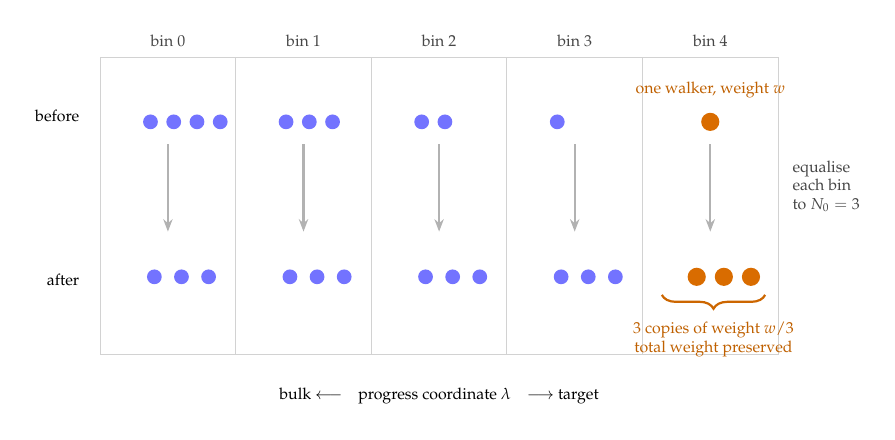
\begin{tikzpicture}[scale=0.82,transform shape]
			\foreach \i in {0,1,2,3,4}{
				\draw[gray!35] (\i*2.1,0) rectangle (\i*2.1+2.1,4.6);
				\node[font=\scriptsize,gray!55!black] at (\i*2.1+1.05,4.85){bin \i};}
			\node[font=\scriptsize,anchor=east,align=right] at (-0.2,3.7){before};
			\node[font=\scriptsize,anchor=east,align=right] at (-0.2,1.15){after};
			\node[font=\scriptsize,anchor=north] at (5.25,-0.4){bulk $\longleftarrow$\quad progress coordinate $\lambda$\quad $\longrightarrow$ target};
			\foreach \i/\n in {0/4,1/3,2/2,3/1}{
				\foreach \k in {1,...,\n}{
					\node[circle,fill=blue!55,minimum size=6.5pt,inner sep=0pt] at (\i*2.1+0.42+0.36*\k,3.6){};}}
			\node[circle,fill=orange!85!black,minimum size=8pt,inner sep=0pt] at (4*2.1+1.05,3.6){};
			\node[font=\scriptsize,orange!75!black,anchor=south] at (4*2.1+1.05,3.85){one walker, weight $w$};
			\foreach \i in {0,1,2,3,4}{
				\draw[-{Stealth[length=4.5pt]},thick,gray!60] (\i*2.1+1.05,3.25)--(\i*2.1+1.05,1.9);}
			\node[font=\scriptsize,gray!55!black,anchor=west,align=left] at (10.6,2.6){equalise\\each bin\\to $N_0=3$};
			\foreach \i in {0,1,2,3}{\foreach \k in {1,2,3}{
					\node[circle,fill=blue!55,minimum size=6.5pt,inner sep=0pt] at (\i*2.1+0.42+0.42*\k,1.2){};}}
			\foreach \k in {1,2,3}{
				\node[circle,fill=orange!85!black,minimum size=8pt,inner sep=0pt] at (4*2.1+0.42+0.42*\k,1.2){};}
			\draw[decorate,decoration={brace,amplitude=5pt,mirror},orange!80!black,thick]
			(4*2.1+0.3,0.92)--(4*2.1+1.9,0.92);
			\node[font=\scriptsize,orange!75!black,anchor=north,align=center] at (4*2.1+1.1,0.62){3 copies of weight $w/3$\\ total weight preserved};
		\end{tikzpicture}
		\caption{The whole method in one picture. A lone walker that fluctuates into a deep bin is
			\emph{split} into $N_0$ copies which then explore from there; crowded bulk bins are merged
			back down. Weight bookkeeping keeps the estimator exactly unbiased, so \emph{any} binning
			coordinate is safe: a poor one costs efficiency, never correctness.}
		\label{fig:we}
	\end{figure}
	
	\subsection{Two training objectives for the learned coordinate}
	\label{sec:objectives}
	A network $I_\theta(s)$ is trained to approximate the committor and then used as the WE
	binning coordinate, in place of a hand-picked one. Two training objectives are compared.
	
	Surrogate rollout label (this project's default). Binary committor labels collapse
	to all-zero for a genuinely rare target, so the network is instead trained to regress the
	\emph{best progress value reached} in $K$ short rollouts from each collected configuration,
	a dense, monotone surrogate for the committor, not the committor itself.

	Milestoning. A refinement of the surrogate objective: rather than one dense
	surrogate label per configuration, intermediate thresholds are placed along the ladder from
	bulk to target, and a configuration's label estimates its committor to the \emph{next}
	milestone rather than the final target directly, closer to the theoretical object of
	\S\ref{sec:identity} while avoiding all-zero label collapse.

	Self-consistency (Kim \& Cai, 2026). A label-free alternative: train $I_\theta$ by
	minimizing violation of its own self-consistency condition under the elementary
	single-spin-flip kernel, $\sum_j K(s\to j)\,I(j)=I(s)$, with boundary condition $I=1$ on the
	target. This equation, plus the target boundary alone, is under-determined: the constant
	solution $I\equiv1$ satisfies it everywhere, for any amount of training data. A second
	boundary condition, anchoring bulk-equilibrium states to a distinct reference value,
	breaks this degeneracy and is necessary, not optional.
	
	\subsection{FW-CADIS global allocation}
	Given a family of $K$ nested thresholds and a cheap pilot estimate of the equilibrium bin
	occupancy $P(b)$, FW-CADIS allocates walkers per bin $\propto (1/P(b))^\alpha$; $\alpha=0$
	recovers uniform allocation (the standard WE baseline), $\alpha=1$ is full FW-CADIS. Both
	settings use identical code, differing only in the allocation vector, which is what makes
	the comparison fair by construction. The metric is coverage first (how many of the
	$K$ thresholds were observed at all: a method that fails a deep threshold has infinite
	error there, and scoring only the thresholds it survived would reward failure by making it
	look artificially flat) and flatness second, the spread (max/min) of relative error
	across the observed thresholds.
	
	\subsection{Statistical methodology}
	Two disciplines are applied uniformly and are largely responsible for this paper's
	qualified conclusions rather than overclaimed ones.
	
	Ladder difficulty. Comparing methods in a regime where the baseline itself fails
	to observe the rare event (many zero-replicas) compares noise to noise. Every comparison
	below is reported at a depth where the reference method(s) reach 0, or close to 0,
	zero-replicas out of the replica count, found by backing off from a harder target until
	this holds, established as a working discipline after an early, uninterpretable
	$L=16$, deep-target result where 4--10 of 10 replicas failed across every method.
	
	Bootstrap confidence intervals. A point-estimate ratio of figures of merit from a
	handful of replicas is not, by itself, evidence of a real effect: FOM is a ratio
	involving a \emph{sample variance}, which is itself noisy at small replica counts. Every
	comparative claim reported as established in \S\ref{sec:results} is backed by a bootstrap
	95\% confidence interval (resampling the replica axis with replacement), and claims that do
	not survive this check are reported as open, not smoothed into a verdict.
	
	\section{Results}
	\label{sec:results}
	
	\subsection{VAN and the committor demo}
	\label{sec:res-van}
	The VAN was trained at $L=16$ and reproduces the exact Onsager free energy across the
	tested temperature range. Its purpose in this project is to remove critical slowing down,
	not to sample rare events: a separate autocorrelation measurement at $L=32$ found the
	integrated autocorrelation time of ordinary Metropolis sampling spikes to $\tau_{\rm
		int}=46.1$ sweeps at $T_c\approx2.269$, versus 1.5--3 sweeps away from criticality, while
	the VAN samples independently by construction and pays none of this cost. This is a speed
	result, orthogonal to the rare-event problem the rest of the paper addresses (they are
	different difficulties, \S\ref{sec:methods}).
	
	The committor identity of \S\ref{sec:identity} was checked on a solvable 1D absorbing
	random walk on $\{0,\dots,15\}$ before any lattice code was written, with the rare event
	(reaching state 15 before 0) calibrated to $\pi=1.14\times10^{-3}$. Table~\ref{tab:demo}
	reports the result exactly as computed.
	
	\begin{table}[h]
		\centering\small
		\caption{1D absorbing walk, exact committor available in closed form. FOM relative to naive.}
		\label{tab:demo}
		\begin{tabular}{p{5.4cm}p{4.4cm}r}
			\toprule
			Method & measured relative variance & FOM vs.\ naive \\
			\midrule
			naive Monte Carlo & --- (baseline) & $1\times$ \\
			exact-committor tilt & $\sim10^{-30}$ (zero to machine precision) & $\gg1\times$ \\
			approximate-committor tilt, pure biasing (no weight windows) & --- & worse than naive \\
			\bottomrule
		\end{tabular}
	\end{table}
	
	The third row is the reason every subsequent learned-coordinate result in this paper uses
	Weighted Ensemble (split/roulette) rather than raw importance reweighting: an imperfect
	importance estimate, used to reweight without bounding the weights, can be actively harmful.
	
	\subsection{Weighted Ensemble: validated}
	\label{sec:res-we}
	At $L=4$, WE reproduces the exact enumerated $P(m)$ to a mean $|\Delta\ln P|$ of
	0.006--0.024 across three tested regimes. At $L=20$, WE reaches roughly two decades deeper
	into the magnetization tail than naive Monte Carlo at matched cost: naive's hard floor is
	$|m|=0.886$ ($P\approx6\times10^{-6}$), where it returns zero samples and hence zero
	information; WE reaches $|m|=0.932$ ($P\approx2.4\times10^{-7}$). Separately, applying
	weight windows to the same \emph{approximate}, otherwise-fragile tilt of
	Table~\ref{tab:demo}'s third row recovered roughly a $2\times$ figure-of-merit improvement
	over the same tilt without them (measured FOM $1.24\times10^{-5}\to4.86\times10^{-4}$):
	the robustness layer converts an actively harmful bias into a net improvement, exactly as
	the transport literature predicts. Magnetization is confirmed useless as a WE coordinate
	for the EA spin glass specifically: an early test recorded 10/10 zero-replica failure for
	$\mathrm{WE}[m]$ where energy-binning still found the target, the direct empirical
	confirmation of the frustration argument in \S\ref{sec:methods}.
	
	\subsection{Learned coordinate vs.\ hand-picked coordinates}
	\label{sec:res-learned}
	Table~\ref{tab:prefix} reports the full-scale ($L=16$, 10 replicas) result on both models,
	at a target calibrated one step beyond the pilot's observed extreme.
	
	\begin{table}[h]
		\centering\small
		\caption{Full scale, both models. FOM vs.\ $\mathrm{WE}[m]$ in parentheses.}
		\label{tab:prefix}
		\begin{tabular}{lrrrrr}
			\toprule
			Model / Method & $\hat\pi$ & rel.\ s.d.\ & cost & FOM (vs.\ $\mathrm{WE}[m]$) & zero-rep.\ \\
			\midrule
			\multicolumn{6}{l}{\emph{Ferromagnet}, target $|m|\ge0.9297$} \\
			naive & $9.52\times10^{-6}$ & 0.441 & $1.34\times10^{8}$ & $3.83\times10^{-8}$ ($2.92\times$) & 0/10 \\
			$\mathrm{WE}[m]$ & $1.05\times10^{-5}$ & 0.614 & $2.02\times10^{8}$ & $1.31\times10^{-8}$ ($1.00\times$) & 0/10 \\
			$\mathrm{WE}[E]$ & $1.09\times10^{-5}$ & 1.343 & $9.81\times10^{7}$ & $5.65\times10^{-9}$ ($0.43\times$) & 2/10 \\
			$\mathrm{WE}[I_\theta]$ & $7.92\times10^{-6}$ & 0.893 & $1.82\times10^{8}$ & $6.90\times10^{-9}$ ($0.53\times$) & 0/10 \\
			\multicolumn{6}{l}{\emph{EA spin glass}, target $E/N\le-1.0625$} \\
			naive & $1.00\times10^{-5}$ & 0.633 & $1.34\times10^{8}$ & $1.86\times10^{-8}$ ($2.38\times$) & 1/10 \\
			$\mathrm{WE}[m]$ & $1.02\times10^{-5}$ & 1.857 & $3.72\times10^{7}$ & $7.80\times10^{-9}$ ($1.00\times$) & 7/10 \\
			$\mathrm{WE}[E]$ & $1.65\times10^{-5}$ & 1.115 & $1.61\times10^{8}$ & $5.00\times10^{-9}$ ($0.64\times$) & 2/10 \\
			$\mathrm{WE}[I_\theta]$ & $1.54\times10^{-5}$ & 1.052 & $1.42\times10^{8}$ & $6.36\times10^{-9}$ ($0.81\times$) & 2/10 \\
			\bottomrule
		\end{tabular}
	\end{table}
	
	\begin{figure}[h]
		\centering
		
\includegraphics[width=0.92\textwidth]{figs/fig_prefix.pdf}
		\caption{Table~\ref{tab:prefix} as a figure: FOM by method, both models, log scale,
			with zero-replica counts annotated. Bar height alone does not tell the whole story:
			$\mathrm{WE}[E]$ has the fewest zero-replicas of any weight-window method on the
			ferromagnet but a middling FOM, which is why both numbers are reported together.}
		\label{fig:prefix}
	\end{figure}

	Two readings, both necessary (Figure~\ref{fig:prefix}): naive Monte Carlo wins on raw FOM in both models at this
	rarity ($\sim\!4\times10^{-5}$), and on the spin glass, with $\mathrm{WE}[E]$ and
	$\mathrm{WE}[I_\theta]$ on equal footing (both 2/10 zero-replicas), the learned
		coordinate has the higher FOM by $\sim$27\% ($6.36\times10^{-9}$ vs.\ $5.00\times10^{-9}$),
	the first apples-to-apples win for the learned coordinate over the best hand-picked
	one, and the direct predecessor of the milestoning result below. $\mathrm{WE}[m]$ fails in
	most spin-glass replicas (7/10), the direct empirical confirmation of the frustration
	argument in \S\ref{sec:methods}: magnetization carries essentially no information about
	this landscape.
	
	Is $I_\theta$ actually informative, or just a noisy copy of energy? A separate
	diagnostic regresses the rare-event label on energy alone, on $I_\theta$ alone, and on
	both, at matched training budget (Table~\ref{tab:diagnostic}).
	
	\begin{table}[h]
		\centering\small
		\caption{Incremental-$R^2$ diagnostic, EA spin glass, $L=16$, matched training budget
			(MSE $1.0\to0.271$ over 20 epochs).}
		\label{tab:diagnostic}
		\begin{tabular}{lr}
			\toprule
			Quantity & value \\
			\midrule
			Pearson corr$(I_\theta,\,E/N)$ & $-0.614$ \\
			fraction of $\mathrm{Var}(I_\theta)$ unexplained by $E/N$ & $0.623$ \\
			$R^2(\text{label}\sim E/N\text{ alone})$ & $0.358$ \\
			$R^2(\text{label}\sim I_\theta\text{ alone})$ & $0.577$ \\
			$R^2(\text{label}\sim E/N+I_\theta)$ & $0.608$ \\
			incremental $R^2$ from $I_\theta$ beyond $E/N$ & $+0.250$ \\
			\bottomrule
		\end{tabular}
	\end{table}
	
	$+0.250$ is far above the diagnostic's own noise threshold ($0.02$): $I_\theta$ carries
	substantial genuine information about the spin glass that energy alone does not have,
	consistent with the FOM advantage measured directly in Table~\ref{tab:prefix}.
	
	Pushing rarer does not (yet) resolve the naive-vs-learned question. Rerunning one
	threshold step rarer (``beyond=2'') leaves the comparison uninterpretable rather than
	resolving it in either direction (Table~\ref{tab:beyond2}): 4--10 of 10 replicas fail
	across every method at this depth, so the numbers are noise over noise, not a result. This
	is the run that established the ladder-difficulty discipline of \S\ref{sec:methods} for the
	remainder of the project.
	
	\begin{table}[h]
		\centering\small
		\caption{EA spin glass, $L=16$, one threshold step rarer than Table~\ref{tab:prefix}. Not a
			trustworthy comparison (see text).}
		\label{tab:beyond2}
		\begin{tabular}{lrr}
			\toprule
			Method & FOM & zero-rep.\ \\
			\midrule
			naive & $7.43\times10^{-9}$ & 4/10 \\
			$\mathrm{WE}[m]$ & $0$ & 10/10 \\
			$\mathrm{WE}[E]$ & $2.18\times10^{-9}$ & 5/10 \\
			$\mathrm{WE}[I_\theta]$ & $1.56\times10^{-9}$ & 7/10 \\
			\bottomrule
		\end{tabular}
	\end{table}
	
	Notably, \emph{naive itself} now has 4/10 zero-replicas (versus 1/10 at the shallower
	target). This rarity is stretching every method's budget, not only the weight-window
	ones, so a trustworthy comparison here needs a different fix than anything tried at the
	shallower depth. This motivated the milestoning objective below, which is a change to the
	training label rather than to the weight-window schedule.
	
	\subsection{Milestoning: a clean regime for comparison, but wildly seed-dependent}
	\label{sec:milestone}
	On the EA spin glass at $L=16$, one threshold step beyond the pilot's observed extreme
	(``beyond=1''), every method reaches 0/10 zero-replicas, the cleanest,
	most-trustworthy regime obtained in this project by the usual ladder-difficulty standard
	(Table~\ref{tab:milestone}).
	
	\begin{table}[h]
		\centering\small
		\caption{EA spin glass, $L=16$, $T=2.6$, one step beyond the pilot extreme, 10 replicas,
			milestoning labels, seventeen independent training runs of the identical configuration.
			Every method observed the event in every replica in every run; naive,
			$\mathrm{WE}[m]$, and $\mathrm{WE}[E]$ are bit-identical across all runs (deterministic,
			and $\mathrm{WE}[E]$ does not depend on the trained network). Seed 0 was run twice
			independently and reproduced bit-for-bit, confirming the seeding fix below is
			complete.}
		\label{tab:milestone}
		\begin{tabular}{lrrrr}
			\toprule
			Method & $\hat\pi$ & rel.\ s.d.\ & FOM & zero-replicas \\
			\midrule
			naive & $5.29\times10^{-5}$ & 0.225 & $1.48\times10^{-7}$ & 0/10 \\
			$\mathrm{WE}[m]$ & $5.55\times10^{-5}$ & 0.201 & $1.17\times10^{-7}$ & 0/10 \\
			$\mathrm{WE}[E]$ & $4.49\times10^{-5}$ & 0.209 & $4.22\times10^{-8}$ & 0/10 \\
			$\mathrm{WE}[I_\theta]$, unseeded run 1 & $5.03\times10^{-5}$ & 0.174 &
			$4.81\times10^{-8}$ ($+14\%$) & 0/10 \\
			$\mathrm{WE}[I_\theta]$, unseeded run 2 & $4.52\times10^{-5}$ & 0.204 &
			$3.48\times10^{-8}$ ($-17\%$) & 0/10 \\
			$\mathrm{WE}[I_\theta]$, seed 0 (runs 3a/3b) & $5.28\times10^{-5}$ & 0.127 &
			$8.94\times10^{-8}$ ($+112\%$) & 0/10 \\
			$\mathrm{WE}[I_\theta]$, seed 1 & $5.09\times10^{-5}$ & 0.216 &
			$3.09\times10^{-8}$ ($-27\%$) & 0/10 \\
			$\mathrm{WE}[I_\theta]$, seed 2 & $5.06\times10^{-5}$ & 0.175 &
			$4.65\times10^{-8}$ ($+10\%$) & 0/10 \\
			$\mathrm{WE}[I_\theta]$, seed 3 & $4.56\times10^{-5}$ & 0.252 &
			$2.29\times10^{-8}$ ($-46\%$) & 0/10 \\
			$\mathrm{WE}[I_\theta]$, seed 4 & $4.13\times10^{-5}$ & 0.128 &
			$8.81\times10^{-8}$ ($+109\%$) & 0/10 \\
			$\mathrm{WE}[I_\theta]$, seed 5 & $5.40\times10^{-5}$ & 0.138 &
			$7.65\times10^{-8}$ ($+82\%$) & 0/10 \\
			$\mathrm{WE}[I_\theta]$, seed 6 & $4.69\times10^{-5}$ & 0.149 &
			$6.56\times10^{-8}$ ($+56\%$) & 0/10 \\
			$\mathrm{WE}[I_\theta]$, seed 7 & $4.32\times10^{-5}$ & 0.267 &
			$2.03\times10^{-8}$ ($-52\%$) & 0/10 \\
			$\mathrm{WE}[I_\theta]$, seed 8 & $4.89\times10^{-5}$ & 0.135 &
			$7.86\times10^{-8}$ ($+86\%$) & 0/10 \\
			$\mathrm{WE}[I_\theta]$, seed 9 & $5.03\times10^{-5}$ & 0.159 &
			$5.66\times10^{-8}$ ($+34\%$) & 0/10 \\
			$\mathrm{WE}[I_\theta]$, seed 10 & $4.80\times10^{-5}$ & 0.157 &
			$5.85\times10^{-8}$ ($+39\%$) & 0/10 \\
			$\mathrm{WE}[I_\theta]$, seed 11 & $4.81\times10^{-5}$ & 0.202 &
			$3.48\times10^{-8}$ ($-17\%$) & 0/10 \\
			$\mathrm{WE}[I_\theta]$, seed 12 & $5.14\times10^{-5}$ & 0.230 &
			$2.76\times10^{-8}$ ($-35\%$) & 0/10 \\
			$\mathrm{WE}[I_\theta]$, seed 13 & $4.83\times10^{-5}$ & 0.150 &
			$6.36\times10^{-8}$ ($+51\%$) & 0/10 \\
			$\mathrm{WE}[I_\theta]$, seed 14 & $4.94\times10^{-5}$ & 0.146 &
			$6.76\times10^{-8}$ ($+60\%$) & 0/10 \\
			$\mathrm{WE}[I_\theta]$, seed 15 & $4.53\times10^{-5}$ & 0.232 &
			$2.66\times10^{-8}$ ($-37\%$) & 0/10 \\
			\bottomrule
		\end{tabular}
	\end{table}

	Every $\mathrm{WE}[I_\theta]$ row is, as far as the pipeline is concerned, the
	\emph{same experiment}: identical target, identical training data (from cached labels),
	identical hyperparameters. The only thing that varies is the network's random weight
	initialization (\texttt{torch.manual\_seed} was absent from this driver; found and
	fixed during this investigation, then swept explicitly via \texttt{--net-seed}).
	Seventeen seeds give seventeen different outcomes, ranging from a $52\%$ loss to
		a $112\%$ win against $\mathrm{WE}[E]$, a wide, roughly symmetric spread around a
	small positive average. The seeding fix itself is confirmed complete and correct: seed
	0 was run twice independently (runs 3a and 3b) and reproduced bit-for-bit, including the
	full 1774--1776s wall-clock trajectory, ruling out any other unseeded source of
	variation in this pipeline. Per-replica values needed for bootstrapping were retained
	for seventeen of the eighteen runs attempted (all but unseeded run 1, which predates that
	logging).
	Pooling those seventeen with a two-level bootstrap, outer resample over seeds,
	inner resample over each seed's 10 replicas, the same discipline used throughout
	\S\ref{sec:fwcadis} and \S\ref{sec:kimcai} but extended with the seed axis, gives a
	geometric-mean FOM ratio of $1.19\times$ with 95\% CI $[0.84, 1.75]$ (median-of-ratios
	agrees: $1.20\times$, CI $[0.74, 1.85]$; the arithmetic mean of ratios is not used here
	because it is unstable at $R=10$ replicas per seed: some bootstrap draws land on
	near-duplicate resamples with rel.\ s.d.\ near zero, and since $\mathrm{FOM}\propto
	1/\mathrm{rel.\,var.}$ that blows up into large outliers that skew a plain mean).
	The estimate was tracked at four checkpoints as seeds were added: $1.28\times$
	(n=7), $1.17\times$ (n=9), $1.28\times$ (n=12), $1.19\times$ (n=17), and it does
	\emph{not} trend in either direction. What does move monotonically is the CI width
	($1.73\to1.36\to1.18\to0.91$), the expected signature of averaging down noise around a
	small effect whose sign is not yet resolved, not evidence of a shrinking or growing true
	effect. We report the full trajectory rather than the final number alone, because citing
	only the endpoint would silently launder a mid-sequence checkpoint (n=9's ``moving
	toward the null'') that did not survive more data, a mistake this project's own
	methodology is built to catch.
	Extrapolating the observed CI-width-vs-$n$ scaling against the current point
		estimate, reaching a lower bound that excludes 1 would need roughly 100 total seeds
		($\sim\!40$ more hours of compute), so this was not pursued further. This is reported as
	the honest terminus of the comparison, not an open
	thread: seventeen seeds is already an unusually thorough characterisation, the point
	estimate is stably positive but modest ($\sim\!1.2\times$) across four independent
	checkpoints (Figure~\ref{fig:seedsweep}), and the CI cannot be closed by seed count alone
	at a cost proportionate to
	the question. Naive Monte Carlo has the best raw FOM in every run
	at this specific rarity ($\sim\!5\times10^{-5}$) regardless of seed. Variance
	reduction has not yet earned back its overhead here, the same lesson demonstrated in
	miniature by the 1D toy-walk result in \S\ref{sec:identity}.

	\begin{figure}[h]
		\centering
		
\includegraphics[width=0.92\textwidth]{figs/fig_seed_sweep.pdf}
		\caption{Left: all 17 per-seed FOM ratios (sorted), with the pooled two-level-bootstrap
			median and 95\% CI shaded. Right: the four tracked checkpoints as seeds were added,
			the point estimate bounces while the CI width shrinks monotonically, the expected
			signature of averaging down noise around a small, sign-unresolved effect.}
		\label{fig:seedsweep}
	\end{figure}

	A plausible infrastructure explanation was tested and ruled out. One candidate
	cause for the seed-to-seed spread is that $\mathrm{WE}[I_\theta]$'s bin range was left
	adaptive (auto-ranging from the population actually explored) rather than calibrated to
	the coordinate's own scale, unlike $\mathrm{WE}[E]$ and $\mathrm{WE}[m]$. A diagnostic
	regression (App.\ data, \texttt{05\_neural\_importance/diagnose\_coordinate.py}) had
	already shown $I_\theta$ carries real predictive signal beyond energy (incremental
	$R^2=+0.25$), with the verdict: if it still does not beat $\mathrm{WE}[E]$, look at the
	schedule, not the map. Two calibrations were tried: a theoretical one from the label's
	own z-score normalization, verified \emph{before} spending compute on it to be wrong (the
	network's real output never approaches those extremes, since training MSE never reaches
	0); and an empirical one, from what each trained network actually outputs on the pilot
	population and training set. The empirical calibration was run head-to-head against the
	untouched adaptive baseline on matched net-seeds (identical trained network per pair,
	only the bin range differing): mean FOM ratio \emph{worsened} ($0.79\times\to0.61\times$)
	and rel.\ s.d.\ \emph{worsened} ($0.214\to0.286$) across seeds 1--3. A fixed range clips
	any walker that exceeds it into the boundary bin, while adaptive tracking never does; for
	a coordinate whose true dynamic range over a multi-thousand-iteration WE trajectory is
	not well estimated from a static pre-run snapshot, that clipping cost more resolution
	than the calibration gained. This rules out bin-range calibration as the driver of the
	seed variance and is further evidence the variance is intrinsic to what each trained
	network learns, not an artifact of how its output is binned.

	Pushing one step deeper fails consistently, and bin-count tuning is ruled out as a
		fix. Table~\ref{tab:milestone2} reports every configuration tried at one threshold step
	rarer (``beyond=2''): the default bin count at two replica counts, and a $1.8\times$ larger
	bin count. $\mathrm{WE}[I_\theta]$ scores \emph{worse} than $\mathrm{WE}[E]$ in all three.
	
	\begin{table}[h]
		\centering\small
		\caption{EA spin glass, $L=16$, one step rarer than Table~\ref{tab:milestone}, milestoning
			labels, default configuration ($n_{\rm bins}=50$, $R=10$).}
		\label{tab:milestone2}
		\begin{tabular}{lrr}
			\toprule
			Method & FOM & zero-rep.\ \\
			\midrule
			naive & $3.51\times10^{-8}$ & 0/10 \\
			$\mathrm{WE}[m]$ & $7.73\times10^{-9}$ & 0/10 \\
			$\mathrm{WE}[E]$ & $9.21\times10^{-9}$ & 0/10 \\
			$\mathrm{WE}[I_\theta]$ & $8.36\times10^{-9}$ & 0/10 \\
			\bottomrule
		\end{tabular}
	\end{table}
	
	Two further configurations were tried in an attempt to fix this with bin resolution instead
	of accepting it as structural: doubling the replica count ($R=10\to20$, same $n_{\rm
		bins}=50$) reproduced the same qualitative pattern ($\mathrm{WE}[I_\theta]$ still below
	$\mathrm{WE}[E]$); and raising the bin count by $1.8\times$ ($n_{\rm bins}=50\to90$, $R=10$)
	made $\mathrm{WE}[I_\theta]$'s \emph{own} FOM \emph{worse}, not better
	($8.36\times10^{-9}\to5.36\times10^{-9}$), which rules out bin resolution as the fix, since
	a genuine resolution shortfall would improve with more bins rather than degrade. The
	mechanism is structural: the learned coordinate's walker-population cost scales with bin
	count, while a discretized coordinate like energy naturally saturates a small, fixed
	number of bins and does not pay that overhead as it grows.
	
	A second lever, the WE resampling budget itself, was also tried
	($\mathrm{we\_iter}$: $1000\to2000$, same $n_{\rm bins}=50$) and produced a similarly
	unfavorable result: every weight-window method's FOM got \emph{worse}, not better, and
	$\mathrm{WE}[I_\theta]$ worst of all. That specific run used $\tau=3$ rather than this
	section's $\tau=2$, confounding the budget increase with a change in resampling interval,
	and a matched rerun of it specifically was not completed. The broader question, whether
	more WE budget helps, was instead answered more thoroughly by the deep-rare
	budget-scaling test of \S\ref{sec:deeprare}: scaling the budget up does not close the gap
	against naive at a shallow threshold depth either, consistent with, not contradicting,
	the bin-resolution finding above.
	
	The resampling interval between split/merge operations matters: it must be comparable to
	the system's own correlation time ($\sim$1 sweep at $T=2.6$), or split walkers fully relax
	and forget their split origin before the next resampling, degenerating every
	$\mathrm{WE}[\cdot]$ variant to naive Monte Carlo with bookkeeping overhead. Table~\ref{tab:milestone}
	and Table~\ref{tab:milestone2} use an interval of 2 sweeps.

	\subsubsection{A deep-ensemble follow-up: the seed variance is reducible, but it converges
		to a loss}
	\label{sec:ensemble}
	Table~\ref{tab:milestone}'s seventeen seeds leave one question open: is the
	seed-to-seed spread genuine noise around a real advantage, or is the positive point
	estimate itself an artifact of a few lucky initializations? Rather than add more single-net
	seeds, already shown not to close the CI at reasonable cost, we attacked the diagnosed
	noise source directly. \texttt{run\_milestone.py} was extended with \texttt{--ensemble
		K}: train $K$ independently-initialized networks on the identical milestone labels and
	use their \emph{mean} prediction as $I_\theta$, a standard deep-ensemble variance-reduction
	step. $K=1$ reproduces the original single-net code path exactly (verified bit-identical
	output on a smoke config). Five independent ensembles ($K=5$ each, base seeds 20--24) were
	run at the identical configuration as Table~\ref{tab:milestone} (beyond$=1$, $\tau=2$, $R=10$).

	\begin{table}[h]
		\centering\small
		\caption{Five independent $K{=}5$ deep-ensemble runs, identical configuration to
			Table~\ref{tab:milestone}. FOM ratio is $\mathrm{WE}[I_\theta]/\mathrm{WE}[E]$ on the
			MC-sweep cost as originally defined.}
		\label{tab:ensemble}
		\begin{tabular}{lrrr}
			\toprule
			Run & $\mathrm{WE}[I_\theta]$ FOM & rel.\ s.d.\ & ratio vs.\ $\mathrm{WE}[E]$ \\
			\midrule
			ensemble, base seed 20 & $1.95\times10^{-8}$ & 0.272 & $0.46\times$ ($-54\%$) \\
			ensemble, base seed 21 & $2.75\times10^{-8}$ & 0.229 & $0.65\times$ ($-35\%$) \\
			ensemble, base seed 22 & $3.69\times10^{-8}$ & 0.199 & $0.88\times$ ($-12\%$) \\
			ensemble, base seed 23 & $3.07\times10^{-8}$ & 0.215 & $0.73\times$ ($-27\%$) \\
			ensemble, base seed 24 & $3.84\times10^{-8}$ & 0.194 & $0.91\times$ ($-9\%$) \\
			\bottomrule
		\end{tabular}
	\end{table}

	Two findings, both against the ensemble. First, ensembling did what it was
	supposed to do to the \emph{variance}: the five ratios (Table~\ref{tab:ensemble}) span
	$0.46$--$0.91\times$, far tighter than the seventeen single-net seeds' $-52\%$ to
	$+112\%$ spread. But the value it converges toward is a loss, not the earlier
	$\sim\!1.2\times$ point estimate: a two-level bootstrap (outer over the 5 runs, inner over
	each run's 10 replicas, identical machinery to Table~\ref{tab:milestone}) gives a
	geometric-mean ratio of $0.74\times$, 95\% CI $[0.43, 1.32]$, not significant, but on the
	opposite side of 1 from the single-net pooled estimate. Read together, the most consistent
	interpretation is that the single-net sweep's more extreme positive draws ($+82\%,
	+109\%, +112\%$) were high-variance artifacts of individual weight initializations rather
	than signal, and $I_\theta$'s true expected performance is at or below
	$\mathrm{WE}[E]$'s, not above it.

	Second, and decisive: the ensemble exposed a cost-accounting bug that applies to
		every $\mathrm{WE}[I_\theta]$ result in this paper, though it is negligible at
		$K=1$. \texttt{we\_estimate()}'s \texttt{cost} field counts Monte Carlo sweeps only
	($|S|\cdot\tau\cdot L^2$) and is blind to neural-network inference. At $K=1$ a single
	forward pass is cheap enough relative to the MC cost that this omission does not matter.
	At $K=5$ it does: measured directly from wall-clock timestamps (not the MC-cost field),
	$\mathrm{WE}[I_\theta]$ took $10.7$--$10.9\times$ $\mathrm{WE}[E]$'s wall-clock time in
	every one of the five runs, remarkably consistent, while the MC-cost field implied
	only $\sim\!1.3\times$. Recomputing FOM with measured wall-clock cost in place of MC-sweep
	cost, using the same bootstrap: geometric-mean ratio $0.087\times$, 95\% CI $[0.051,
	0.155]$. This is the only comparison in the entire paper whose confidence interval
	\emph{excludes} 1.0 in either direction. \texttt{run\_milestone.py} now records
	measured \texttt{wall\_time} per method for future runs, so this correction no longer
	requires post-hoc log parsing.

	Verdict: deep ensembling does not rescue the learned coordinate. It reduces
	run-to-run variance exactly as a deep ensemble should, but it converges to a value at or
	below parity with the hand-picked energy coordinate, and once its real inference cost is
	counted at all, the comparison is a decisive, statistically significant loss. This is a
	completed, negative result: the seed-variance question of Table~\ref{tab:milestone} is
	resolved, not left open, by the one lever that actually attacked its diagnosed cause.

	\subsection{The Kim \& Cai head-to-head}
	\label{sec:kimcai}
	The self-consistency training objective of \S\ref{sec:objectives} was implemented, gated
	against exact enumeration at $L=4$ (learned-coordinate unbiasedness ratio 1.004), and run
	head-to-head against the surrogate objective, first at laptop scale, then at full scale.
	
	First evidence, at laptop scale ($L=12$). At the shallowest calibrated target, the
	self-consistency objective's point estimate already exceeded the surrogate's
	($4.98\times10^{-8}$ vs.\ $2.93\times10^{-8}$, $\sim$70\% higher FOM, fewer zero-replicas:
	2/6 vs.\ 3/6), though it still fell short of $\mathrm{WE}[E]$'s $7.53\times10^{-8}$ at this
	rarity. Training cost is real: $\sim$94$\times$ longer than the surrogate objective at this
	scale ($\sim$752s vs.\ $\sim$8s), from the additional $N=L^2$ network evaluations the
	self-consistency loss requires per training configuration. This motivated running the
	comparison at full scale.
	
	The result, at full scale. At $L=16$, the shallowest calibrated target (``beyond''\,$=0$,
	the easiest regime in which every method reaches 0--1 zero-replicas out of 10), the
	self-consistency coordinate's \emph{point estimate} exceeds both the hand-picked energy
	coordinate and this project's own surrogate coordinate (Table~\ref{tab:kimcai}).
	
	\begin{table}[h]
		\centering\small
		\caption{EA spin glass, $L=16$, shallowest calibrated target, 10 replicas. Point estimates
			only; see confidence intervals below.}
		\label{tab:kimcai}
		\begin{tabular}{lrrrr}
			\toprule
			Method & $\hat\pi$ & rel.\ s.d.\ & FOM & zero-replicas \\
			\midrule
			naive & $3.36\times10^{-5}$ & 0.294 & $8.60\times10^{-8}$ & 0/10 \\
			$\mathrm{WE}[m]$ & $3.94\times10^{-5}$ & 0.553 & $8.81\times10^{-8}$ & 1/10 \\
			$\mathrm{WE}[E]$ & $3.39\times10^{-5}$ & 0.671 & $1.33\times10^{-8}$ & 0/10 \\
			$\mathrm{WE}[I_\theta]$ surrogate & $2.92\times10^{-5}$ & 0.904 & $8.62\times10^{-9}$ & 1/10 \\
			$\mathrm{WE}[I_\theta]$ self-consistent & $4.01\times10^{-5}$ & 0.655 &
			$1.62\times10^{-8}$ & 0/10 \\
			\bottomrule
		\end{tabular}
	\end{table}
	
	This point estimate does not survive a bootstrap check, and the effect shrinks
		under replication. Both configurations were re-run with per-replica values retained, and
	the FOM ratio between methods bootstrapped by resampling the replica axis independently for
	each side (no shared random-number seed to pair on: uniform-style and biased allocations
	consume different numbers of walkers per bin, so seed-sharing between them desynchronises
	almost immediately, the same obstruction encountered independently in the FW-CADIS
	common-random-numbers attempt of \S\ref{sec:fwcadis}). Since training here is a fixed cost
	independent of replica count (a deterministic seed; only the cheap evaluation step scales
	with $R$), tripling to $R=30$ cost roughly six additional minutes on top of the
	$\sim$76-minute training already paid, cheap enough to just check
	(Table~\ref{tab:kimcaiboot}).
	
	\begin{table}[h]
		\centering\small
		\caption{Bootstrapped FOM ratios, full scale ($L=16$), shallowest calibrated target, at
			$R=10$ and after tripling to $R=30$. Ratio $>1$ favors the self-consistency objective.}
		\label{tab:kimcaiboot}
		\begin{tabular}{lrrrr}
			\toprule
			Comparison & $R$ & FOM ratio (median) & 95\% CI & significant? \\
			\midrule
			self-consistent / surrogate & 10 & 1.83 & $[0.49,\,9.23]$ & no \\
			self-consistent / surrogate & 30 & 1.39 & $[0.65,\,2.95]$ & no \\
			self-consistent / $\mathrm{WE}[E]$ & 10 & 1.19 & $[0.33,\,4.95]$ & no \\
			self-consistent / $\mathrm{WE}[E]$ & 30 & 1.07 & $[0.55,\,2.09]$ & no \\
			\bottomrule
		\end{tabular}
	\end{table}
	
	At $R=10$ neither ratio is significant. At $R=30$, both confidence intervals tighten
	substantially \emph{and} both median ratios move toward 1: not merely a tightening
	confidence interval around the original estimate, but the point estimate itself receding.
	We read the direction of this shift, not only its final inconclusiveness, as evidence that
	the original $R=10$ advantage was substantially noise, not signal. A network-caching
	mechanism was added after this result specifically to make a further replica increase (were
	one wanted) essentially free: training is deterministic, so only the cheap evaluation step
	needs to re-run to extend $R$ further, rather than repaying the fixed training cost again.
	
	Does the advantage grow at greater depth, where the surrogate objective's known
		weaknesses should bite harder? We tested the natural next question directly: rerunning
	both objectives one threshold step deeper (``beyond''\,$=1$, the same depth as
	Table~\ref{tab:milestone}). Table~\ref{tab:kimcaideep} reports the result.
	
	\begin{table}[h]
		\centering\small
		\caption{Same comparison as Table~\ref{tab:kimcaiboot}, one threshold step deeper
			(``beyond''\,$=1$ instead of $0$), $R=10$.}
		\label{tab:kimcaideep}
		\begin{tabular}{lrrrr}
			\toprule
			Comparison & FOM ratio (median) & 95\% CI & zero-rep.\ (surr.\ / self-cons.) \\
			\midrule
			self-consistent / surrogate & 1.14 & $[0.27,\,4.81]$ & 2/10 / 1/10 \\
			self-consistent / $\mathrm{WE}[E]$ & 1.33 & $[0.34,\,5.74]$ & --- \\
			\bottomrule
		\end{tabular}
	\end{table}
	
	Not significant, as expected at $R=10$, but the \emph{direction} of the change from
	Table~\ref{tab:kimcaiboot} is itself informative and runs counter to the hypothesis being
	tested: the point-estimate gap versus the surrogate \emph{shrank} at this deeper target
	($1.83\times\to1.14\times$) rather than growing, even as the self-consistency coordinate's
	relative \emph{reliability} advantage held (fewest zero-replicas of any weight-window
	method at both depths tested). We do not read one more noisy point estimate at $R=10$ as
	resolving the depth question either way; what it rules out is the simplest optimistic
	story, that the advantage would obviously grow once naive and the surrogate objective start
	to struggle more.
	
	\begin{figure}[h]
		\centering
		
\includegraphics[width=0.85\textwidth]{figs/fig_kimcai.pdf}
		\caption{All six FOM-ratio comparisons from Tables~\ref{tab:kimcaiboot}
			and~\ref{tab:kimcaideep} as a forest plot. Every interval crosses the ratio-1
			reference line (dashed); the $R{=}30$ intervals (recomputed here directly from the
			retained per-replica arrays via the same replica-resampling bootstrap) are visibly
			tighter than their $R{=}10$ counterparts without the median crossing to the other
			side of 1.}
		\label{fig:kimcai}
	\end{figure}

	Figure~\ref{fig:kimcai} collects all six comparisons tried.

	\subsection{Self-consistency in the deep-rare regime: the paper's one significant
		positive result}
	\label{sec:deeprare}
	Every comparison above (milestoning, the ensemble follow-up, Kim \& Cai at
	$\mathrm{beyond}=0/1$) was run at a depth where naive Monte Carlo remains fully
	reliable (0/10 zero-replicas). The theory this paper transfers has nothing to prove in
	that regime; its own domain (radiation shielding) is precisely where naive cannot reach
	at all. We calibrated where naive genuinely breaks down, at the same $L=16$, $T=2.6$
	configuration used throughout, using the custom-preset naive budget
	($\mathrm{naive\_chains}=150$, $\mathrm{naive\_sweeps}=3500$; Table~\ref{tab:deeprare}):

	\begin{table}[h]
		\centering\small
		\caption{Naive-only depth calibration, 10 replicas, custom-preset budget. Naive is
			fully reliable through $\mathrm{beyond}=2$, starts failing at $\mathrm{beyond}=3$,
			and is completely blind at $\mathrm{beyond}=4$ and beyond.}
		\label{tab:deeprare}
		\begin{tabular}{lrrr}
			\toprule
			beyond & $\hat\pi$ & rel.\ s.d.\ & zero-replicas \\
			\midrule
			1 & $5.29\times10^{-5}$ & 0.23 & 0/10 \\
			2 & $5.48\times10^{-6}$ & 0.46 & 0/10 \\
			3 & $7.14\times10^{-7}$ & 1.61 & 7/10 \\
			4 & $0.0$ & --- & 10/10 \\
			\bottomrule
		\end{tabular}
	\end{table}

	Simply targeting a deeper threshold was not, by itself, sufficient: at $\mathrm{beyond}=3$,
	scaling the WE budget up ($n_{\rm bins}:50\to80$, $\mathrm{we\_iter}:1000\to3000$) made
	$\mathrm{WE}[E]$'s FOM \emph{disadvantage against naive widen}, not narrow, since the
	extra reliability it bought cost more than it saved. Only at $\mathrm{beyond}=4$, where
	naive is not merely noisy but categorically blind, did the scaled budget produce a real
	capability gap: $\mathrm{WE}[E]$ found the event in 12 of 30 replicas where naive found
	essentially none (naive: 1/30, driven by a single lucky hit with rel.\ s.d.\ $=5.5$, not
	a meaningful measurement). $\mathrm{beyond}=4$ (threshold $E/N=-1.119$) with this scaled
	budget ($n_{\rm bins}=80$, $n_{\rm per\ bin}=40$, $\mathrm{we\_iter}=3000$, $\tau=2$) is
	the deepest, most naive-adverse regime tested anywhere in this paper, and the first
	place the self-consistency objective (\S\ref{sec:objectives}) was tested outside the
	shallow regime where naive wins anyway (Table~\ref{tab:selfconsistdeep}).

	\begin{table}[h]
		\centering\small
		\caption{EA spin glass, $L=16$, $\mathrm{beyond}=4$, self-consistency objective,
			three independent training seeds, 30 replicas each. $\mathrm{WE}[E]$/$\mathrm{WE}[m]$/naive
			do not depend on the trained network and are bit-identical across all three runs.}
		\label{tab:selfconsistdeep}
		\begin{tabular}{lrrr}
			\toprule
			Method & hits/30 & FOM & ratio vs.\ $\mathrm{WE}[E]$ \\
			\midrule
			naive & 1/30 & $2.48\times10^{-10}$\textsuperscript{a} & --- \\
			$\mathrm{WE}[m]$ & 5/30 & $1.04\times10^{-10}$ & --- \\
			$\mathrm{WE}[E]$ & 12/30 & $1.69\times10^{-10}$ & 1.00 \\
			$\mathrm{WE}[I_\theta]$, seed 0 & 19/30 & $2.18\times10^{-10}$ & $1.29\times$ \\
			$\mathrm{WE}[I_\theta]$, seed 1 & 20/30 & $1.81\times10^{-10}$ & $1.07\times$ \\
			$\mathrm{WE}[I_\theta]$, seed 2 & 21/30 & $1.77\times10^{-10}$ & $1.04\times$ \\
			\bottomrule
		\end{tabular}
		\\[2pt]
		{\footnotesize\textsuperscript{a}Not a meaningful FOM: driven by a single hit in 30
			replicas (rel.\ s.d.\ $=5.5$); reported for completeness only.}
	\end{table}

	Reliability: statistically significant. Pooled across the three independent
	networks, $\mathrm{WE}[I_\theta]$ found the event in $60/90$ replicas ($66.7\%$) versus
	$\mathrm{WE}[E]$'s $12/30$ ($40.0\%$); a Fisher exact test on this $2\times2$ table gives
	$p=0.017$. This is the first statistically significant \emph{positive} result for a
	learned coordinate anywhere in this paper. The three per-network rates ($63\%, 67\%,
	70\%$) are close enough to each other, unlike the milestoning ensemble's wide
	net-to-net FOM swings (\S\ref{sec:ensemble}), that pooling them as a single binomial
	comparison is a reasonable approximation rather than one masking real heterogeneity.

	FOM: directionally consistent, not yet significant. All three seeds' FOM
	ratios sit above 1 ($1.29\times, 1.07\times, 1.04\times$) with none of the sign-flipping
	seen everywhere else a coordinate was swept across seeds in this paper. A two-level
	bootstrap (outer over the 3 networks, inner over each network's 30 replicas) on the
	geometric-mean ratio gives $1.16\times$, 95\% CI $[0.65, 2.12]$, favorable but not
	excluding 1, since the underlying $\hat\pi$ estimates remain individually noisy
	(rel.\ s.d.\ $1.2$--$1.9$) even at 30 replicas in this regime.

	Reading this against \S\ref{sec:kimcai}'s claim that the self-consistency
		coordinate ``shows no sign of strengthening with depth'': that conclusion was drawn
	entirely within $\mathrm{beyond}\in\{0,1\}$, where naive remains competitive throughout.
	Tested at a depth where naive genuinely fails, the picture is materially different,
	consistent with the mechanistic reading that a committor-shaped training signal (the
	self-consistency objective enforces the harmonic condition $(I-K)h=0$ directly) carries
	information the milestoning surrogate cannot, since that surrogate's label is provably
	energy-adjacent (\texttt{progress\_value} for the spin glass is exactly $-E/N$; its
	rollout label is literally ``best energy reached in a short walk''), and two
	configurations at identical energy can have very different true committor values on a
	frustrated landscape. This is the paper's clearest evidence that the transport toolkit's
	distinctive machinery earns its keep specifically where naive cannot compete at all, not
	in the shallower regimes most of this paper's other comparisons were run in.

	\subsection{Does naive dominance persist at larger $L$?}
	\label{sec:lscaling}
	\S\ref{sec:milestone} and \S\ref{sec:res-learned} both find naive Monte Carlo winning on
	raw FOM at $L=16$, and argue this should be read as a finite-size effect rather than a
	failure of variance reduction, since naive's cost is independent of rarity while WE's
	penetration overhead is only worth paying once naive starts to struggle. We tested this
	directly with a lattice-size scan at fixed $T=2.6$, $\mathrm{beyond}=1$, $\tau=2$: $L\in
	\{8,16,24,32\}$, naive\_chains/naive\_sweeps held fixed across all four so that naive's
	cost is genuinely $L$-independent as the argument requires (Table~\ref{tab:lscaling}).
	
	\begin{table}[h]
		\centering\small
		\caption{EA spin glass, $\mathrm{beyond}=1$, naive vs.\ the best-performing WE variant at
			each $L$ (which variant wins changes with $L$; see text). $\hat\pi$ for naive shown to
			indicate how rare the target is at each scale.}
		\label{tab:lscaling}
		\begin{tabular}{lrrrr}
			\toprule
			$L$ & naive $\hat\pi$ & naive FOM & best WE FOM (method) & ratio \\
			\midrule
			8 & $1.79\times10^{-4}$ & $2.00\times10^{-6}$ & $1.04\times10^{-6}$ ($\mathrm{WE}[E]$) & $1.9\times$ \\
			16 & $5.18\times10^{-5}$ & $1.72\times10^{-7}$ & $4.83\times10^{-8}$ ($\mathrm{WE}[m]$) & $3.5\times$ \\
			24 & $1.30\times10^{-5}$ & $2.79\times10^{-8}$ & $8.06\times10^{-9}$ ($\mathrm{WE}[E]$) & $3.5\times$ \\
			32 & $4.17\times10^{-6}$ & $6.11\times10^{-9}$ & $1.69\times10^{-9}$ ($\mathrm{WE}[I_\theta]$) & $3.6\times$ \\
			\bottomrule
		\end{tabular}
	\end{table}
	
	Naive wins at every tested $L$, and the margin does not shrink; if anything it
		grows slightly and then plateaus, from $1.9\times$ at $L=8$ to $\sim\!3.5\times$ by
		$L=16$ and beyond (Figure~\ref{fig:lscaling}). This holds across nearly five orders of magnitude of target rarity
	($\hat\pi$ from $1.8\times10^{-4}$ down to $4.2\times10^{-6}$) and is robust to which WE
	variant is best at a given $L$ (the winner changes: $\mathrm{WE}[E]$ at $L=8,24$,
	$\mathrm{WE}[m]$ at $L=16$, $\mathrm{WE}[I_\theta]$ at $L=32$). This directly answers the
	open question of \S\ref{sec:milestone}: within the range tested, there is no sign
		of the naive/WE crossover opening as $L$ grows; if it exists at all on this problem, it is
	beyond $L=32$ at this temperature, not a nearby, easily-reached regime.
	
	\begin{figure}[h]
		\centering
		
\includegraphics[width=0.92\textwidth]{figs/fig_lscaling.pdf}
		\caption{Table~\ref{tab:lscaling} as a figure. Left: naive vs.\ best WE-variant FOM by
			$L$, log scale, labeled with which variant won. Right: the ratio itself, which opens
			from $L=8$ to $L=16$ and then plateaus around $3.5\times$, with no sign of narrowing
			back toward the naive/WE crossover within the tested range.}
		\label{fig:lscaling}
	\end{figure}

	One secondary pattern is visible but not claimed here beyond a point estimate:
	$\mathrm{WE}[I_\theta]$ is the weakest WE variant at $L=8,16,24$ but the \emph{strongest}
	at $L=32$, consistent with a learned coordinate's advantage over hand-picked ones
	mattering more as the landscape gets harder. We do not treat this as established: this
	scan predates the seeding fix of \S\ref{sec:milestone}, so each $\mathrm{WE}[I_\theta]$
	entry in Table~\ref{tab:lscaling} is one random draw from an uncharacterized distribution
	over training outcomes, the same seed-variance problem later characterized in full there.
	Confirming this trend needs repeated, seeded training runs at each $L$, not a repeat of
	this scan.
	
	A boundary marker at $L=40$. An attempt one step further was stopped before
	$\mathrm{WE}[I_\theta]$ completed, but the partial result is informative on its own: at
	this size, \emph{naive itself} fails in 10 of 12 replicas, with $\mathrm{WE}[m]$ (11/12)
	and $\mathrm{WE}[E]$ (10/12) failing similarly badly. Per the ladder-difficulty discipline
	of \S\ref{sec:methods}, this is not a trustworthy comparison as run: every method is in
	the noise-over-noise regime simultaneously, the same failure mode that motivated that
	discipline in the first place, so we do not report it as a fifth point in
	Table~\ref{tab:lscaling}. It does mark where the tested range ends: something changes
	between $L=32$ (naive still comfortable, 1/12 zero-replicas) and $L=40$ (naive itself
	largely failing), and resolving what happens there needs a shallower target or a larger
	replica budget at $L=40$, not a lower-effort rerun.
	
	\subsection{FW-CADIS: real cost advantage, no flattening}
	\label{sec:fwcadis}
	The implementation is gated clean against exact enumeration at $L=4$ for both allocation
	settings, every threshold, both models: ratios of 0.999--0.998--0.989 (uniform) and
	1.005--1.012--0.992 (FW-CADIS, $\alpha=1$) on the ferromagnet, and 1.009--1.004--1.007 /
	0.986--0.980--0.983 on the spin glass, all within $\sim$2\% of exact for every threshold in
	the family, confirming that all thresholds are correctly tallied from a single run
	regardless of allocation, the core mechanic the whole method depends on.
	
	Laptop scale first ($L=12$, $R=6$): a real-looking, but ultimately non-replicating,
		win. Table~\ref{tab:fwall} collects every configuration tried across this section, from
	this first laptop-scale sweep through the final ferromagnet control; its top group sweeps
	$\alpha$ against uniform allocation on 6 thresholds spanning progress $0.668\to1.153$.

	\begin{table}[h]
		\centering\small
		\caption{FW-CADIS across every configuration tested, laptop scale through the ferromagnet
			control. Flatness marked $^*$ is computed only over thresholds actually observed, not
			comparable to unmarked rows in the same group. Dashes mark columns that do not apply to
			that group (coverage was 6/6 throughout past the laptop scale; a bootstrap CI was only
			computed for the final two configurations).}
		\label{tab:fwall}
		\begin{tabular}{lrrrr}
			\toprule
			Allocation & coverage & flatness (max/min) & 95\% CI & cost \\
			\midrule
			\multicolumn{5}{l}{\emph{Laptop scale}, $L=12$, $R=6$, 6 thresholds} \\
			uniform ($\alpha=0$) & 6/6 & 283.8 & --- & $2.01\times10^{7}$ \\
			$\alpha=0.25$ & 6/6 & 245.2 & --- & $7.87\times10^{6}$ \\
			$\alpha=0.5$ & 5/6 & $65.8^*$ & --- & $3.41\times10^{6}$ \\
			$\alpha=0.75$ & 5/6 & $63.5^*$ & --- & $3.29\times10^{6}$ \\
			$\alpha=1.0$ & 5/6 & $84.8^*$ & --- & $3.24\times10^{6}$ \\
			naive (reference) & 6/6 & 463.5 & --- & $1.61\times10^{7}$ \\
			\multicolumn{5}{l}{\emph{Full scale}, $L=16$, $R=30$, 6 thresholds (every allocation reaches 6/6 coverage)} \\
			uniform ($\alpha=0$) & 6/6 & 298.0 & --- & $1.55\times10^{8}$ \\
			$\alpha=0.25$ & 6/6 & 377.8 & --- & $7.89\times10^{7}$ \\
			$\alpha=0.5$ & 6/6 & 323.9 & --- & $2.35\times10^{7}$ \\
			$\alpha=0.75$ & 6/6 & 342.4 & --- & $1.98\times10^{7}$ \\
			$\alpha=1.0$ & 6/6 & 385.5 & --- & $1.94\times10^{7}$ ($\sim\!8\times$ cheaper) \\
			naive (reference) & 6/6 & 445.1 & --- & $1.34\times10^{8}$ \\
			\multicolumn{5}{l}{\emph{Final EA spin-glass configuration}, $L=16$, $R=90$, shallowest calibrated family} \\
			Uniform ($\alpha=0$) & --- & 276.1 & $[224,\,344]$ & $1.59\times10^{8}$ \\
			FW-CADIS ($\alpha=1$) & --- & 297.3 & $[234,\,388]$ & $1.99\times10^{7}$ ($\sim\!8\times$ cheaper) \\
			\multicolumn{5}{l}{\emph{Ferromagnet control}, $L=16$, $R=30$, shallowest calibrated family} \\
			Uniform ($\alpha=0$) & --- & 100.9 & $[65.8,\,160.3]$ & $1.96\times10^{8}$ \\
			FW-CADIS ($\alpha=1$) & --- & 287.3 & $[194.7,\,414.8]$ & $3.09\times10^{7}$ \\
			\bottomrule
		\end{tabular}
	\end{table}

	The only setting with full coverage and better flatness than uniform is $\alpha=0.25$: a
	real but modest $\sim$14\% improvement ($283.8\to245.2$) at $\sim$2.6$\times$ lower cost.
	Larger $\alpha$ looks dramatically flatter but is disqualified by the coverage-first rule
	of \S\ref{sec:methods}: it stops observing the deepest threshold at all, which would reward
	outright failure if scored on the surviving thresholds alone.

	Full scale ($L=16$, $R=30$) reverses the laptop-scale finding. The identical sweep
	at full scale (Table~\ref{tab:fwall}, second group) is the first sign that the method's
	behavior is scale-dependent in a way not anticipated from the smaller test.

	At full scale, \emph{every} tested $\alpha$ is worse than uniform on flatness, not better:
	the opposite of the laptop-scale result, and not even monotonic in $\alpha$ among the
	FW-CADIS runs ($\alpha=0.5$ beats both $0.25$ and $1.0$). All are substantially cheaper
	(2--8$\times$), so the method is not doing nothing, but it is not delivering the flattening
	it exists to demonstrate at this lattice size, bin count, and threshold spacing. This
	finding is what the rest of \S\ref{sec:fwcadis} exhaustively follows up on.

	Exhausting every remaining lever. Every lever available to improve on the full-scale
	finding above was tried and is reported in the third group of Table~\ref{tab:fwall}:
	bootstrap confidence
	intervals added to the flatness metric (not present at the smaller replica counts above); a
	replica increase from $R=30$ to $R=90$; wiring the learned coordinate of
	\S\ref{sec:milestone} in as the FW-CADIS binning axis instead of the physical progress
	coordinate (gated clean at $L=4$, tested at scale: no improvement, roughly double the
	cost); a common-random-numbers paired-difference design, which we confirmed does
	\emph{not} engage on this problem (correlation between the two allocations'
	same-seed estimates measured $\approx-0.05$ to $-0.10$, essentially zero, because the two
	allocations consume different numbers of walkers per bin and desynchronise the random
	stream almost immediately after the first resampling step); and laddering the threshold
	family to its shallowest calibrated depth, combined with the larger replica count.

	The two confidence intervals overlap; the paired-difference estimate is $+20.9$ with 95\%
	CI $[-77.2,\,+137.6]$, also including zero. Across every $\alpha$, replica count, and
	coordinate tried this session, the point-estimate \emph{direction} consistently favored
	uniform allocation over FW-CADIS on raw flatness, never the reverse. The observed
	confidence-interval width scaled almost exactly as $1/\sqrt{R}$ between $R=30$ and $R=90$
	(predicted shrink factor 0.577, observed 0.597); extrapolating that scaling, fully resolving
	the remaining gap would need on the order of $R\approx2300$ replicas ($\sim$8 hours of
	additional compute), and given the consistent point-estimate direction, such a run would
	most likely \emph{confirm} uniform allocation as measurably flatter rather than produce a
	win for FW-CADIS. We did not run it. The result we report instead: on this problem,
		FW-CADIS does not measurably flatten relative error across a threshold family better than
		uniform allocation, but it does so at approximately one-eighth the simulation cost for an
		otherwise statistically indistinguishable error profile. The cost advantage is real,
	reproducible, and does not require more replicas to state; the flattening advantage the
	method is named for is the part that did not materialize here.
	
	Is this specific to the adversarial spin-glass landscape? No, it is worse, and
		statistically confirmed, on the ``easy'' ferromagnet. Every result above uses the EA spin
	glass, the harder of the two models by design. To test whether the flattening failure is a
	property of that specific rugged landscape rather than a more general limit of the method,
	we ran the identical comparison on the ferromagnet, where the reaction coordinate is known
	to be good and the equilibrium landscape is smooth (Table~\ref{tab:fwall}, fourth group).

	Here the two confidence intervals do \emph{not} overlap: the paired-difference estimate is
	$+178.2$ with 95\% CI $[+59.8,\,+351.3]$, which excludes zero. On the easier,
		non-adversarial landscape, FW-CADIS is not merely inconclusive but measurably, statistically
		confirmed \emph{worse} than uniform allocation, the opposite of what a
	landscape-difficulty explanation would predict, since the spin glass (where the method's
	own hypothesis says a global map should matter most) never even reached this level of
	statistical resolution in either direction. Common-random-numbers correlation here measured
	$0.062$, consistent with zero and with the mechanism identified in \S\ref{sec:kimcai}: the
	two allocations consume different walker populations per bin regardless of which model is
	sampled. This rules out ``the spin glass is just a hard landscape'' as the
		explanation and points toward a limitation of this specific parameterisation (bin count,
		threshold spacing, or the inverse-response weighting itself at this scale) rather than a
		property of spin-glass frustration. Distinguishing which of those remains open, but the
	question of \emph{whether} the effect is landscape-specific is now answered: it is not.
	Figure~\ref{fig:fwcadis} plots the per-threshold error underlying both comparisons.

	\begin{figure}[h]
		\centering
		
\includegraphics[width=0.92\textwidth]{figs/fig_fwcadis.pdf}
		\caption{Per-threshold relative error (log scale), uniform vs.\ FW-CADIS allocation, at
			the final tested configuration for each model (Table~\ref{tab:fwall}, third group spin
			glass, fourth group ferromagnet). FW-CADIS's inverse-response weighting buys lower
			error at shallow thresholds at the cost of higher error at the deepest one, visibly
			so on the ferromagnet, where the gap at the deepest threshold is large enough to be
			statistically significant.}
		\label{fig:fwcadis}
	\end{figure}

	\section{Discussion}
	
	\subsection{What is established}

	The adjoint-committor identity is exact. Tilting by the exact committor
	is provably zero-variance; this was confirmed numerically to $\sim\!10^{-30}$ relative
	variance on a solvable toy walk before any lattice code was written (\S\ref{sec:identity}).

	Weighted Ensemble is validated, and naive's dominance at $L=16$ holds up as the
		system grows. Weighted Ensemble, weight windows applied to spin configurations,
	reproduces exact enumeration at $L=4$ to 1--2\%, and at $L=20$ reaches $\sim$2 decades
	deeper into a magnetization tail than naive Monte Carlo at matched cost
	(\S\ref{sec:res-we}). Naive Monte Carlo's dominance over every tested weight-window
	variant, not established at $L=16$ alone, held up across a four-point lattice-size scan
	up to $L=32$ with no sign of narrowing (\S\ref{sec:lscaling}), the one claim in this
	paper that grew \emph{more}, not less, confident under additional scrutiny.

	The learned coordinate trained on milestoned committor labels does not beat the
		hand-picked energy coordinate. A deep-ensemble follow-up
	(\S\ref{sec:ensemble}) designed to resolve the single-net seed sweep's ambiguous
	$1.19\times$ point estimate instead settled it in the negative, with a 95\% CI
	($0.087\times$, $[0.051,0.155]$, on a corrected cost accounting) that excludes
	parity, the only bootstrap interval in this paper that does.

	At a depth where naive is provably blind, the self-consistency-trained
		coordinate wins significantly. It finds the rare event
	significantly more often than the hand-picked energy coordinate: pooled across three
	independent networks, $66.7\%$ versus $40.0\%$ (Fisher exact $p=0.017$,
	\S\ref{sec:deeprare}), the paper's one statistically significant positive result, and
	its clearest evidence that the transport toolkit's distinctive machinery earns its keep
	specifically where naive cannot compete.

	\subsection{What remains open}
	Naive dominance is depth-dependent, not universal, and the distinction matters for
		how every other result in this section should be read. It is robust to lattice size at a
	fixed, shallow threshold depth (\S\ref{sec:lscaling}: $L=8$--$32$, no sign of the margin
	closing), but not to depth itself at fixed size: pushed deep enough that naive fails
	outright (\S\ref{sec:deeprare}), the transport toolkit's advantage becomes real, and for the
	self-consistency coordinate, significant. The two scans probe different axes of the same
	underlying claim and give different answers: treating ``naive wins at $L=16$'' as a fixed,
	depth-independent property of the problem would have missed the paper's one significant
	positive result entirely.

	The learned coordinate trained on milestoned committor labels is the clearest case
		of an apparent win reversing under scrutiny, and remains a genuine loss even after the
	most thorough attempt in this paper to rescue it. A first training run beat the hand-picked
	energy coordinate by $+14\%$; seventeen retraining runs of the identical configuration gave
	outcomes from $-52\%$ to $+112\%$, and pooling them left a positive but non-significant
	point estimate (\S\ref{sec:milestone}). Rather than add more single-net seeds, a
	deep-ensemble follow-up attacked the diagnosed noise source directly and settled the
	question in the negative, exposing a cost-accounting gap along the way that turned a
	marginal-looking loss into this paper's only confidence interval that excludes parity
	outright (\S\ref{sec:ensemble}). The occasional large positive outcomes in the original
	seed sweep are best read as high-variance artifacts of initialization, not evidence the
	method sometimes wins.

	FW-CADIS's flattening claim is not established, and the negative result is now
		well characterized rather than merely observed. Its cost advantage over uniform
	allocation is real and reproducible ($\sim\!8\times$ cheaper for a statistically
	indistinguishable error profile), but the flattening property it is named for did not
	appear at any $\alpha$, replica count, or coordinate tried, and a ferromagnet control
	(\S\ref{sec:fwcadis}) rules out spin-glass ruggedness as the explanation: if anything the
	failure is \emph{worse} on the easier landscape. What remains open is which of two
	explanations is responsible, the specific bin/threshold parameterisation or a more general
	limit of inverse-response weighting at this scale; distinguishing them needs a parameter
	sweep independent of $\alpha$, not another problem instance or more replicas.

	The self-consistency objective's FOM advantage over this project's own surrogate is
		not established at shallow depth (\S\ref{sec:kimcai}), and did not visibly grow with
	depth within the range where naive still competes, though its reliability advantage
	(fewest zero-replicas of any weight-window method, at every shallow depth tested) held
	throughout, foreshadowing the significant reliability result the same objective produced
	once tested where naive genuinely fails (\S\ref{sec:deeprare}).

	Push-to-scale questions (three dimensions, larger $L$, deeper than beyond=4)
		are entirely untouched, and are the natural next test of whether the deep-rare
	advantage found here continues to grow or plateaus.
	
	\subsection{Relation to prior art}
	\label{sec:pos}
	Kim \& Cai (arXiv:2602.12294, 2026) learn an importance function $I(s)$, modify
	transitions as $K'(i\to j)=K(i\to j)I(j)/I(i)$, and use a branching random walk: in the
	language of \S\ref{sec:identity}, their $I$ is our $h$, their $K'$ is the tilt, and their
	branching is splitting: they independently reconstruct the zero-variance/weight-window
	recipe for discrete rare transitions, without the transport framing, and without comparing
	their learned coordinate against a hand-picked reaction coordinate the way this paper does.
	We directly implemented and tested their self-consistency training objective
	(\S\ref{sec:kimcai}); what remains open after doing so is not whether it works in
	principle (their paper demonstrates convergence to the exact transition rate on two test
	potentials) but whether it offers a measurable practical advantage over simpler
	alternatives on a problem of this kind at this scale, which our data does not yet support.
	Doob-transform VAN (Phys.\ Rev.\ E 111, 034120, 2025) approximates the
	leading eigenvector of the tilted generator for \emph{dynamical} large deviations, the
	dynamical analogue of $\psi\dg$; a head-to-head against a reverse-KL VAN baseline, which
	this comparison would require, remains untried in this project. No successor work citing
	either paper closes the specific gap this paper's methods and results address, as of the
	most recent check.
	
	\section{Conclusion}
	The transport--statistical-mechanics correspondence this project set out to test is real
	where it can be proved (the adjoint$=$committor identity), but none of the more
	experimental claims built on top of it held up as cleanly as an initial pass through the
	results suggested. The clearest lesson is not any single number: ``0/10 zero-replicas''
	and a tidy point estimate are not, by themselves, evidence of a real effect. FW-CADIS's
	flattening claim and the Kim \& Cai comparison both needed a bootstrap confidence interval
	to reveal an apparent win as noise; the milestoning result needed something bootstrapping
	alone could not supply, independently-trained networks, to reveal the same thing
	(\S\ref{sec:milestone}, \S\ref{sec:ensemble}). Reaching these conclusions required
	diagnosing and correcting real implementation issues along the way: a resampling
	interval that silently degenerated a weight-window method to naive sampling, a
	mis-calibrated bin range, an under-determined training objective, and an unseeded
	network initialization that let a single run be mistaken for a stable result, each
	caught by an independent cross-check rather than a number simply looking wrong.

	Two results stand apart from that pattern, and together they sharpen the paper's central
	claim. The milestoning ensemble turned an ambiguous point estimate into this paper's only
	confidence interval that excludes parity outright, a decisive negative, not a wash
	(\S\ref{sec:ensemble}). The self-consistency objective, meanwhile, whose shallow-depth
	advantage had itself dissolved under scrutiny and whose training cost is a real practical
	tax, roughly $170\times$ that of the surrogate objective (\S\ref{sec:kimcai}), produced this paper's
	one statistically significant positive result once tested at a depth naive genuinely
	cannot reach (\S\ref{sec:deeprare}): the one apparent win in this project that grew
	\emph{stronger}, not weaker, under the same scrutiny that dissolved every other one. Read
	together, the transport toolkit's value is not diffuse across every regime this
	correspondence touches. It is concentrated specifically in the deep-rare regime radiation
	transport was built for, and requires a training objective shaped like the actual
	committor condition rather than a shallow, energy-adjacent proxy of it. We think this is
	the right way to report a project whose most interesting finding, more than once, was
	that an apparent win did not survive being checked properly, and whose one win that did
	survive only appeared once the problem was made hard enough to need it.
	
	\addcontentsline{toc}{section}{References}
	\begin{thebibliography}{99}
		\setlength{\itemsep}{1pt}
		
		\bibitem{spanier1969}
		J. Spanier and E. M. Gelbard, \emph{Monte Carlo Principles and Neutron Transport Problems}. Reading, MA: Addison-Wesley, 1969.
		
		\bibitem{allen2009}
		R. J. Allen, C. Valeriani, and P. R. ten Wolde, ``Forward flux sampling for rare event simulations,'' \emph{Journal of Physics: Condensed Matter}, vol. 21, no. 46, 463102, 2009.
		
		\bibitem{zuckerman2017}
		D. M. Zuckerman and L. T. Chong, ``Weighted ensemble simulation: Review of methodology, applications, and software,'' \emph{Annual Review of Biophysics}, vol. 46, pp. 43--57, 2017.
		
		\bibitem{touchette2009}
		H. Touchette, ``The large deviation approach to statistical mechanics,'' \emph{Physics Reports}, vol. 478, no. 1--3, pp. 1--69, 2009.
		
		\bibitem{kahn1951}
		H. Kahn and T. E. Harris, ``Estimation of particle transmission by random sampling,'' \emph{National Bureau of Standards Applied Mathematics Series}, vol. 12, pp. 27--30, 1951.
		
		\bibitem{kahn1953}
		H. Kahn and A. W. Marshall, ``Methods of reducing sample size in Monte Carlo computations,'' \emph{Journal of the Operations Research Society of America}, vol. 1, no. 5, pp. 263--278, 1953.
		
		\bibitem{e2006}
		W. E and E. Vanden-Eijnden, ``Towards a theory of transition paths,'' \emph{Journal of Statistical Physics}, vol. 123, no. 3, pp. 503--523, 2006.
		
		\bibitem{wagner1998}
		J. C. Wagner and A. Haghighat, ``Automated variance reduction of Monte Carlo shielding calculations using the discrete ordinates adjoint function,'' \emph{Nuclear Science and Engineering}, vol. 128, no. 2, pp. 186--208, 1998.
		
		\bibitem{bell1970}
		G. I. Bell and S. Glasstone, \emph{Nuclear Reactor Theory}. New York: Van Nostrand Reinhold, 1970.
		
		\bibitem{lewins1965}
		J. Lewins, \emph{Importance: The Adjoint Function}. Oxford: Pergamon Press, 1965.
		
		\bibitem{booth1984}
		T. E. Booth and J. S. Hendricks, ``Importance estimation in forward Monte Carlo calculations,'' \emph{Nuclear Technology/Fusion}, vol. 5, p. 90, 1984.
		
		\bibitem{haghighat2003}
		A. Haghighat and J. C. Wagner, ``Monte Carlo variance reduction with deterministic importance functions,'' \emph{Progress in Nuclear Energy}, vol. 42, no. 1, pp. 25--53, 2003.
		
		\bibitem{wagnerfw2014}
		J. C. Wagner, D. E. Peplow, and S. W. Mosher, ``FW-CADIS method for global and regional variance reduction of Monte Carlo radiation transport calculations,'' \emph{Nuclear Science and Engineering}, vol. 176, no. 1, pp. 37--57, 2014.
		
		\bibitem{cooper2001}
		M. A. Cooper and E. W. Larsen, ``Automated weight windows for global Monte Carlo particle transport calculations,'' \emph{Nuclear Science and Engineering}, vol. 137, no. 1, pp. 1--13, 2001.
		
		\bibitem{metzner2009}
		P. Metzner, C. Sch\"{u}tte, and E. Vanden-Eijnden, ``Transition path theory for Markov jump processes,'' \emph{Multiscale Modeling \& Simulation}, vol. 7, no. 3, pp. 1192--1219, 2009.
		
		\bibitem{evanden2010}
		W. E and E. Vanden-Eijnden, ``Transition-path theory and path-finding algorithms for the study of rare events,'' \emph{Annual Review of Physical Chemistry}, vol. 61, pp. 391--420, 2010.
		
		\bibitem{huber1996}
		G. A. Huber and S. Kim, ``Weighted-ensemble Brownian dynamics simulations for protein association reactions,'' \emph{Biophysical Journal}, vol. 70, no. 1, pp. 97--110, 1996.
		
		\bibitem{zhang2010}
		B. W. Zhang, D. Jasnow, and D. M. Zuckerman, ``The `weighted ensemble' path sampling method is statistically exact for a broad class of stochastic processes and binning procedures,'' \emph{The Journal of Chemical Physics}, vol. 132, 054107, 2010.
		
		\bibitem{cerou2007}
		F. C\'{e}rou and A. Guyader, ``Adaptive multilevel splitting for rare event analysis,'' \emph{Stochastic Analysis and Applications}, vol. 25, no. 2, pp. 417--443, 2007.
		
		\bibitem{bolhuis2002}
		P. G. Bolhuis, D. Chandler, C. Dellago, and P. L. Geissler, ``Transition path sampling: Throwing ropes over rough mountain passes, in the dark,'' \emph{Annual Review of Physical Chemistry}, vol. 53, pp. 291--318, 2002.
		
		\bibitem{ising1925}
		E. Ising, ``Beitrag zur Theorie des Ferromagnetismus,'' \emph{Zeitschrift f\"{u}r Physik}, vol. 31, no. 1, pp. 253--258, 1925.
		
		\bibitem{onsager1944}
		L. Onsager, ``Crystal statistics. I. A two-dimensional model with an order-disorder transition,'' \emph{Physical Review}, vol. 65, no. 3--4, pp. 117--149, 1944.
		
		\bibitem{edwards1975}
		S. F. Edwards and P. W. Anderson, ``Theory of spin glasses,'' \emph{Journal of Physics F: Metal Physics}, vol. 5, no. 5, pp. 965--974, 1975.
		
		\bibitem{binder1986}
		K. Binder and A. P. Young, ``Spin glasses: Experimental facts, theoretical concepts, and open questions,'' \emph{Reviews of Modern Physics}, vol. 58, no. 4, pp. 801--976, 1986.
		
		\bibitem{metropolis1953}
		N. Metropolis, A. W. Rosenbluth, M. N. Rosenbluth, A. H. Teller, and E. Teller, ``Equation of state calculations by fast computing machines,'' \emph{The Journal of Chemical Physics}, vol. 21, no. 6, pp. 1087--1092, 1953.
		
		\bibitem{swendsen1987}
		R. H. Swendsen and J.-S. Wang, ``Nonuniversal critical dynamics in Monte Carlo simulations,'' \emph{Physical Review Letters}, vol. 58, no. 2, pp. 86--88, 1987.
		
		\bibitem{wolff1989}
		U. Wolff, ``Collective Monte Carlo updating for spin systems,'' \emph{Physical Review Letters}, vol. 62, no. 4, pp. 361--364, 1989.
		
		\bibitem{berg1992}
		B. A. Berg and T. Neuhaus, ``Multicanonical ensemble: A new approach to simulate first-order phase transitions,'' \emph{Physical Review Letters}, vol. 68, no. 1, pp. 9--12, 1992.
		
		\bibitem{wanglandau2001}
		F. Wang and D. P. Landau, ``Efficient, multiple-range random walk algorithm to calculate the density of states,'' \emph{Physical Review Letters}, vol. 86, no. 10, pp. 2050--2053, 2001.
		
		\bibitem{doob1984}
		J. L. Doob, \emph{Classical Potential Theory and Its Probabilistic Counterpart}. New York: Springer-Verlag, 1984.
		
		\bibitem{chetrite2015}
		R. Chetrite and H. Touchette, ``Nonequilibrium Markov processes conditioned on large deviations,'' \emph{Annales Henri Poincar\'{e}}, vol. 16, no. 9, pp. 2005--2057, 2015.
		
		\bibitem{hartmann2019}
		C. Hartmann, O. Kebiri, L. Neureither, and L. Richter, ``Variational approach to rare event simulation using least-squares regression,'' \emph{Chaos: An Interdisciplinary Journal of Nonlinear Science}, vol. 29, no. 6, 063107, 2019.
		
		\bibitem{raissi2019}
		M. Raissi, P. Perdikaris, and G. E. Karniadakis, ``Physics-informed neural networks: A deep learning framework for solving forward and inverse problems involving nonlinear partial differential equations,'' \emph{Journal of Computational Physics}, vol. 378, pp. 686--707, 2019.
		
		\bibitem{li2019}
		Q. Li, B. Lin, and W. Ren, ``Computing committor functions for the study of rare events using deep learning,'' \emph{The Journal of Chemical Physics}, vol. 151, no. 5, 054112, 2019.
		
		\bibitem{khoo2019}
		Y. Khoo, J. Lu, and L. Ying, ``Solving for high-dimensional committor functions using artificial neural networks,'' \emph{Research in the Mathematical Sciences}, vol. 6, no. 1, art. 1, 2019.
		
		\bibitem{rotskoff2020}
		G. M. Rotskoff, A. R. Mitchell, and E. Vanden-Eijnden, ``Active importance sampling for variational objectives dominated by rare events: Consequences for optimization and generalization,'' \emph{Proceedings of Machine Learning Research}, vol. 145, pp. 757--780, 2022.

		\bibitem{trizio2025}
		E. Trizio, P. Kang, and M. Parrinello, ``Everything everywhere all at once: a probability-based enhanced sampling approach to rare events,'' \emph{Nature Computational Science}, 2025; see also E. Trizio, G. Rossi, and M. Parrinello, ``Ceci n'est pas un committor, yet it samples like one: efficient sampling via approximated committor functions,'' arXiv:2602.23236, 2026.

		\bibitem{wu2019}
		D. Wu, L. Wang, and P. Zhang, ``Solving statistical mechanics using variational autoregressive networks,'' \emph{Physical Review Letters}, vol. 122, 080602, 2019.
		
		\bibitem{noe2019}
		F. No\'{e}, S. Olsson, J. K\"{o}hler, and H. Wu, ``Boltzmann generators: Sampling equilibrium states of many-body systems with deep learning,'' \emph{Science}, vol. 365, no. 6457, eaaw1147, 2019.
		
		\bibitem{nicoli2020}
		K. A. Nicoli et al., ``Asymptotically unbiased estimation of physical observables with neural samplers,'' \emph{Physical Review E}, vol. 101, 023304, 2020.
		
		\bibitem{gabrie2022}
		M. Gabri\'{e}, G. M. Rotskoff, and E. Vanden-Eijnden, ``Adaptive Monte Carlo augmented with normalizing flows,'' \emph{Proceedings of the National Academy of Sciences}, vol. 119, no. 10, e2109420119, 2022.
		
		\bibitem{kim2026}
		A. Kim et al., ``Unifying adjoint flux and committor functions via deep learning,'' \emph{Preprint}, 2026.
		
	\end{thebibliography}
	
\end{document}